% !TEX program = xelatex
% HeapBeat scientific project report.
\documentclass[12pt,a4paper,twoside,openright]{report}

\usepackage{fontspec}
\defaultfontfeatures{Ligatures=TeX,Scale=MatchLowercase}
\setmainfont{Times New Roman}
\setsansfont{Arial}
\setmonofont[Scale=0.86]{Courier New}
\usepackage{polyglossia}
\setmainlanguage{vietnamese}
\setotherlanguage{english}
\usepackage{setspace}
\usepackage{scrextend}
\changefontsizes{13pt}
\onehalfspacing

\usepackage[a4paper,inner=3cm,outer=2cm,top=2.5cm,bottom=2.5cm,headheight=16pt]{geometry}
\usepackage{graphicx}
\usepackage{booktabs,tabularx,array,multirow}
\usepackage{enumitem}
\usepackage{xcolor}
\usepackage{amsmath,amssymb}
\usepackage{tikz}
\usetikzlibrary{arrows.meta,positioning,shapes.geometric,fit,calc}
\usepackage{pgfgantt}
\usepackage{listings}
\usepackage{fancyhdr}
\usepackage{titlesec}
\usepackage{tocloft}
\usepackage{chngcntr}
\usepackage{hyperref}
\usepackage{microtype}
\usepackage{caption}
\usepackage{float}
\usepackage{longtable}
\usepackage{needspace}
\usepackage{etoolbox}
\usepackage{pdflscape}
\usepackage{emptypage}

\definecolor{hbgreen}{HTML}{087F78}
\definecolor{hbnavy}{HTML}{173C4A}
\definecolor{hbgold}{HTML}{B45309}
\definecolor{hbink}{HTML}{17211F}
\definecolor{hbmuted}{HTML}{50615C}
\definecolor{hbline}{HTML}{DDE5E1}
\definecolor{hblight}{HTML}{F4F8F6}

\hypersetup{
  unicode=true,
  colorlinks=true,
  linkcolor=hbgreen,
  urlcolor=hbnavy,
  pdfdisplaydoctitle=true,
  pdftitle={HeapBeat -- Phát nhạc chờ cộng đồng cho phòng tự học},
  pdfauthor={Nhóm HeapBeat},
  pdfsubject={Báo cáo đồ án Cấu trúc dữ liệu và Giải thuật},
  pdfkeywords={Max-Heap, danh sách liên kết đôi vòng, Hash Map, Collaborative DJ Queue}
}

\pagestyle{fancy}
\fancyhf{}
\fancyhead[LE]{\small\itshape\leftmark}
\fancyhead[RO]{\small\itshape\rightmark}
\fancyfoot[C]{\small\thepage}
\renewcommand{\headrulewidth}{0.4pt}
\renewcommand{\footrulewidth}{0pt}
\renewcommand{\chaptermark}[1]{\markboth{Chương \thechapter.\ #1}{}}
\renewcommand{\sectionmark}[1]{\markright{\thesection\ #1}}
\fancypagestyle{plain}{%
  \fancyhf{}
  \fancyfoot[C]{\small\thepage}
  \renewcommand{\headrulewidth}{0pt}
}

\titleformat{\chapter}[block]
  {\normalfont\Large\bfseries\centering}
  {CHƯƠNG \thechapter.}{0.6em}{\MakeUppercase}
\titlespacing*{\chapter}{0pt}{0pt}{30pt}
\titleformat{\section}
  {\normalfont\large\bfseries}
  {\thesection}{1em}{}
\titlespacing*{\section}{0pt}{12pt}{6pt}
\titleformat{\subsection}
  {\normalfont\normalsize\bfseries}
  {\thesubsection}{1em}{}
\titlespacing*{\subsection}{0pt}{10pt}{4pt}
\titleformat{\subsubsection}
  {\normalfont\normalsize\itshape\bfseries}
  {\thesubsubsection}{1em}{}

\renewcommand{\cftchapfont}{\bfseries}
\renewcommand{\cftchappagefont}{\bfseries}
\renewcommand{\cftchapleader}{\bfseries\cftdotfill{\cftdotsep}}
\setlength{\cftbeforechapskip}{6pt}
\setlength{\cftbeforesecskip}{2pt}

\setlength{\parindent}{1.25cm}
\setlength{\parskip}{0pt}
\AtBeginEnvironment{tabular}{\setlength{\parindent}{0pt}}
\AtBeginEnvironment{tabularx}{\setlength{\parindent}{0pt}}
\AtBeginEnvironment{longtable}{\setlength{\parindent}{0pt}}
\AtBeginEnvironment{minipage}{\setlength{\parindent}{0pt}}
\AtBeginEnvironment{lstlisting}{\setlength{\parindent}{0pt}}
\setlist[itemize]{leftmargin=1.5em,itemsep=2pt,topsep=4pt,parsep=0pt}
\setlist[enumerate]{leftmargin=1.7em,itemsep=2pt,topsep=4pt,parsep=0pt}
\captionsetup{font=small,labelfont=bf,labelsep=period,width=0.92\textwidth,
  skip=5pt,justification=centering}
\renewcommand{\figurename}{Hình}
\renewcommand{\tablename}{Bảng}
\renewcommand{\contentsname}{Mục lục}
\renewcommand{\listfigurename}{Danh mục hình}
\renewcommand{\listtablename}{Danh mục bảng}
\renewcommand{\bibname}{Tài liệu tham khảo}
\emergencystretch=2em
\raggedbottom
\clubpenalty=10000
\widowpenalty=10000
\displaywidowpenalty=10000

\lstdefinestyle{heapbeat}{
  basicstyle=\ttfamily\footnotesize,
  backgroundcolor=\color{hblight},
  frame=single,
  rulecolor=\color{hbline},
  breaklines=true,
  showstringspaces=false,
  columns=fullflexible,
  xleftmargin=4pt,
  xrightmargin=4pt,
  aboveskip=4pt,
  belowskip=4pt
}
\lstset{style=heapbeat}
\AtBeginDocument{\counterwithin{lstlisting}{chapter}}
\lstdefinestyle{algorithm}{
  style=heapbeat,
  numbers=left,
  numberstyle=\ttfamily\scriptsize\color{hbmuted},
  commentstyle=\color{hbgreen!70!black}\itshape,
  numbersep=8pt,
  xleftmargin=1.8em
}

\newcommand{\code}[1]{\texttt{#1}}
\newcommand{\metric}[2]{%
  \begin{minipage}[t]{0.29\linewidth}
  \centering
  {\sffamily\bfseries\Large\color{hbgreen}#1\par}
  {\sffamily\small\color{hbmuted}#2\par}
  \end{minipage}}
\newcommand{\status}[1]{\textcolor{hbgreen}{\sffamily\bfseries #1}}
\newcommand{\pagelead}[1]{\noindent\textcolor{hbmuted}{\small #1}}
\newcommand{\researchq}[2]{%
  \noindent\textbf{#1.} #2\par\smallskip}
\newcommand{\evidencebox}[2]{%
  \begin{center}
  \fcolorbox{hbline}{hblight}{%
    \begin{minipage}{0.92\textwidth}\small
      \textbf{#1.} #2
    \end{minipage}}
  \end{center}}

\begin{document}
\hypersetup{pageanchor=false}
\pagenumbering{gobble}

% PAGE 1 -----------------------------------------------------------------------
\begin{titlepage}
\thispagestyle{empty}
\begin{singlespace}
\centering
\vspace*{-0.45cm}

\includegraphics[width=3.2cm]{logo-khtn.png}\par
\vspace{0.35cm}
{\large\bfseries ĐẠI HỌC QUỐC GIA THÀNH PHỐ HỒ CHÍ MINH\par}
\vspace{0.12cm}
{\large\bfseries TRƯỜNG ĐẠI HỌC KHOA HỌC TỰ NHIÊN\par}
\vspace{0.12cm}
{\normalsize\bfseries KHOA ĐIỆN TỬ -- VIỄN THÔNG\par}

\vspace{1.3cm}
{\LARGE\bfseries BÁO CÁO ĐỒ ÁN\par}
\vspace{0.28cm}
{\large\bfseries HỌC PHẦN CẤU TRÚC DỮ LIỆU VÀ GIẢI THUẬT\par}

\vspace{1.15cm}
{\fontsize{30}{36}\selectfont\bfseries HeapBeat\par}
\vspace{0.3cm}
{\fontsize{21}{27}\selectfont\bfseries
Phát Nhạc Chờ Cộng Đồng\\[0.16cm]
Cho Phòng Tự Học\par}
\vspace{0.16cm}
{\large\bfseries (COLLABORATIVE DJ QUEUE)\par}
\vspace{0.42cm}
{\large\itshape Hệ thống xếp hàng ưu tiên và bình chọn bài hát\par}

\vfill
{\normalsize\bfseries Nhóm sinh viên thực hiện:\par}
\vspace{0.08cm}
{\normalsize\itshape HeapBeat\par}
\vspace{0.18cm}
{\small
\renewcommand{\arraystretch}{1.08}
\begin{tabular}[t]{r @{\quad} l}
24207043 & Phạm Hùng Tiến\\
24207029 & Trần Thái Nguyên\\
24207105 & Quách Gia Thịnh\\
24207110 & Đặng Gia Toàn\\
24207002 & Phạm Cao Bằng\\
24207111 & Lê Quang Bảo Trung\\
24207090 & Văn Phú Duy\\
24207101 & Hồ Sĩ Phú\\
\end{tabular}\par}

\vfill
{\large Thành phố Hồ Chí Minh, ngày 08 tháng 08 năm 2026\par}
\end{singlespace}
\end{titlepage}

% PROJECT INFORMATION ----------------------------------------------------------
\thispagestyle{empty}
\chapter*{Thông tin báo cáo}

\renewcommand{\arraystretch}{1.24}
\begin{tabularx}{\textwidth}{@{}p{3.55cm}X@{}}
\toprule
\textbf{Hạng mục} & \textbf{Thông tin}\\
\midrule
Học phần & Cấu trúc dữ liệu và Giải thuật\\
Loại tài liệu & Báo cáo đồ án khoa học kỹ thuật\\
Đề tài & HeapBeat -- Phát nhạc chờ cộng đồng cho phòng tự học
(Collaborative DJ Queue)\\
Trạng thái & Bản nộp học phần, tháng 8 năm 2026\\
Ngày thuyết trình & 08/08/2026\\
Kho mã nguồn & \href{https://github.com/PhamHungTien/HeapBeat}{github.com/PhamHungTien/HeapBeat}\\
Giấy phép mã nguồn & MIT License\\
Nền tảng & React, TypeScript, Web/PWA; mô hình đối chiếu bằng C11\\
CTDL trọng tâm & Max-Heap + Index Map; danh sách liên kết đôi vòng; Hash Map\\
Kết quả kiểm tra & 22/22 kiểm thử đơn vị đạt; bản C chạy đúng; bản dựng web hoàn tất\\
\bottomrule
\end{tabularx}

\vspace{0.72cm}
{\sffamily\large\bfseries\color{hbnavy}Danh sách nhóm và gói công việc chính\par}
\vspace{0.1cm}
\begin{tabularx}{\textwidth}{@{}p{2.05cm}p{3.75cm}X@{}}
\toprule
\textbf{MSSV} & \textbf{Thành viên} & \textbf{Gói công việc chính}\\
\midrule
24207043 & Phạm Hùng Tiến & Kiến trúc trạng thái, tích hợp và đóng gói\\
24207029 & Trần Thái Nguyên & CDLL và điều khiển Next/Prev/Repeat\\
24207105 & Quách Gia Thịnh & Max-Heap, bộ so sánh, bình chọn và xóa\\
24207110 & Đặng Gia Toàn & SpamGuard, cửa sổ trượt, chặn và thu hồi\\
24207002 & Phạm Cao Bằng & Giao diện thích ứng và khả năng truy cập\\
24207111 & Lê Quang Bảo Trung & Cổng API PHP--C và snapshot JSON\\
24207090 & Văn Phú Duy & Kế hoạch kiểm thử, bản C và tổng hợp số liệu\\
24207101 & Hồ Sĩ Phú & Danh mục nhạc, giấy phép và báo cáo\\
\bottomrule
\end{tabularx}

\vfill
\cleardoublepage

\hypersetup{pageanchor=true}
\pagenumbering{roman}
\setcounter{page}{1}

% FRONT MATTER -----------------------------------------------------------------
\chapter*{Tóm tắt}
\addcontentsline{toc}{chapter}{Tóm tắt}
\markboth{Tóm tắt}{Tóm tắt}
Đề tài xuất phát từ nhu cầu tổ chức một danh sách phát chung trong phòng tự học, nơi nhiều
sinh viên có thể đề xuất và bình chọn bài hát nhưng không được làm gián đoạn trải nghiệm
của những người còn lại. Bài toán đặt ra ba yêu cầu chính: xác định nhanh bài có mức ưu
tiên cao nhất, duyệt lịch sử phát theo hai chiều và hạn chế các yêu cầu lặp lại từ cùng một
tài khoản. Trên cơ sở đó, nhóm xây dựng \textbf{HeapBeat}, một ứng dụng web/PWA sử dụng
Max-Heap kèm bản đồ chỉ số cho hàng đợi bình chọn, danh sách liên kết đôi vòng cho lịch sử
phát và Hash Map theo mã sinh viên cho cơ chế chống gửi yêu cầu quá mức.

Hệ thống dùng React 19 và TypeScript cho giao diện, còn backend C11 là nguồn sự thật thực thi
ba cấu trúc dữ liệu. Độ đúng đắn được xem xét thông qua bất biến,
độ phức tạp tiệm cận, 22 kiểm thử đơn vị, 56 assertion backend C và các tình huống sử dụng
trên trình duyệt. Kết quả cho thấy cả 22 kiểm thử đều đạt; thao tác xem phần tử đầu Heap,
Next/Prev và tra cứu trạng thái chống spam có chi phí $O(1)$ (trung bình đối với Hash Map),
trong khi thêm, lấy, xóa và cập nhật bình chọn có chi phí $O(\log n)$. Ở các kích thước màn
hình đã kiểm tra, bảng hàng đợi không phát sinh cuộn ngang. Báo cáo đồng thời nêu rõ những
giới hạn còn lại về xác thực, đồng bộ nhiều thiết bị và quyền biểu diễn âm nhạc công cộng.

\textbf{Từ khóa:} Max-Heap; hàng đợi ưu tiên; danh sách liên kết đôi vòng; Hash Map;
chống spam; React; PWA; hệ thống phát nhạc cộng đồng.

\cleardoublepage
\chapter*{Abstract}
\addcontentsline{toc}{chapter}{Abstract}
\markboth{Abstract}{Abstract}
Community music-selection systems must efficiently identify the highest-priority track,
support bidirectional playback history, and limit repeated requests from a single user.
This report presents \textbf{HeapBeat}, a web/PWA prototype for self-study rooms. A
Max-Heap with an index map manages the voting queue, a circular doubly linked list models
playback history, and a StudentID-indexed hash map enforces a sliding-window anti-spam
policy. React 19 and TypeScript implement the client, while an authoritative C11 backend
owns the core data structures and exposes their state through a JSON API.

The evaluation combines invariant checking, asymptotic complexity analysis, 22 automated
unit tests, warning-free C compilation, web build verification, and interface checks at
desktop, narrow-laptop, and mobile widths. All 22 tests pass. Heap peek, playlist
Next/Previous, and average hash lookup operate in $O(1)$; insert, extract, arbitrary
removal, and vote updates operate in $O(\log n)$. At the inspected viewports, the queue
introduces no horizontal overflow. The results support the suitability of the selected
data structures for the stated use case, while remaining limited to the scale and
conditions of an academic prototype.

\textbf{Keywords:} Max-Heap; priority queue; circular doubly linked list; hash map;
anti-spam; React; PWA; community music system.

\cleardoublepage
\markboth{Mục lục}{Mục lục}
\tableofcontents
\cleardoublepage
\phantomsection
\addcontentsline{toc}{chapter}{Danh mục hình}
\markboth{Danh mục hình}{Danh mục hình}
\listoffigures
\cleardoublepage
\phantomsection
\addcontentsline{toc}{chapter}{Danh mục bảng}
\markboth{Danh mục bảng}{Danh mục bảng}
\listoftables
\cleardoublepage
\chapter*{Danh mục từ viết tắt và ký hiệu}
\addcontentsline{toc}{chapter}{Danh mục từ viết tắt và ký hiệu}
\markboth{Danh mục từ viết tắt và ký hiệu}{Danh mục từ viết tắt và ký hiệu}
\begin{tabularx}{\textwidth}{@{}p{3.25cm}X@{}}
\toprule
\textbf{Ký hiệu/thuật ngữ} & \textbf{Diễn giải trong báo cáo}\\
\midrule
$H$, $n$ & Mảng lưu Heap và số phần tử hiện hành.\\
$i$, $parent(i)$ & Chỉ số một node và chỉ số node cha trong Heap.\\
CDLL & Circular Doubly Linked List -- danh sách liên kết đôi vòng.\\
RQ & Research Question -- câu hỏi nghiên cứu.\\
Điều kiện kiểm chứng & Tiêu chí độc lập dùng để xác định một ca kiểm thử đúng hay sai.\\
PWA & Progressive Web App -- ứng dụng web có manifest và service worker.\\
TB $O(1)$ & Độ phức tạp trung bình hằng số của thao tác Hash Map.\\
\bottomrule
\end{tabularx}

\cleardoublepage
\pagenumbering{arabic}
\setcounter{page}{1}

% PAGE 2 -----------------------------------------------------------------------
\chapter{Giới thiệu và đặc tả nghiên cứu}
\pagelead{HeapBeat chuyển một bài toán bình chọn quen thuộc thành mô hình trực quan cho ba
cấu trúc dữ liệu trọng tâm: hàng đợi ưu tiên, danh sách liên kết vòng và bảng băm.}

\section{Bài toán}
Tại các không gian công cộng của trường như sảnh hoặc phòng tự học, nhiều sinh viên cùng
đề xuất bài hát. Danh sách phát phải phản ánh lựa
chọn của cộng đồng, vẫn cho phép Next/Prev/Repeat, và không bị một tài khoản chi phối.
HeapBeat cung cấp hai vai trò: \textbf{sinh viên} gửi yêu cầu và bình chọn; \textbf{quản trị viên}
điều khiển trình phát, kiểm duyệt bản quyền, cấu hình phòng và theo dõi sự cố.

\section{Mục tiêu và phương pháp}
Mục tiêu của nghiên cứu là đánh giá mức độ phù hợp của ba cấu trúc dữ liệu đối với một
luồng chọn nhạc cộng đồng, thay vì chứng minh khả năng chịu tải của một dịch vụ thương mại.
Quá trình thực hiện gồm bốn bước: đặc tả yêu cầu và bất biến; xây dựng lõi cấu trúc dữ liệu
độc lập; tích hợp lõi vào ứng dụng; và kiểm tra kết quả bằng các điều kiện đã xác định trước.
Mỗi câu hỏi nghiên cứu được đối chiếu với ít nhất một nhóm kiểm thử đơn vị và một hành vi
có thể quan sát trên giao diện.

Dữ liệu đầu vào bao gồm thứ tự gửi yêu cầu, điểm số, lịch sử bình chọn, thời điểm gửi và
trạng thái của mã sinh viên. Các đại lượng được theo dõi gồm phần tử đầu Heap, thứ tự xếp
hạng, con trỏ lịch sử phát, danh sách yêu cầu bị thu hồi và mã phản hồi của hệ thống. Bộ
dữ liệu minh họa được giữ cố định để các lần chạy có thể lặp lại. Vì chưa thực hiện phép
đo tải quy mô lớn, những nhận định về hiệu năng trong báo cáo chỉ dựa trên phân tích tiệm cận.

\section{Câu hỏi nghiên cứu}
\researchq{RQ1}{Max-Heap có bản đồ chỉ số có duy trì đúng thứ tự ưu tiên sau khi thêm,
thay đổi bình chọn, xóa và lấy phần tử đầu, đồng thời giữ chi phí cập nhật $O(\log n)$ hay không?}
\researchq{RQ2}{Danh sách liên kết đôi vòng có mô hình hóa tự nhiên Next, Previous và Repeat All
với chi phí $O(1)$ và xử lý đúng các trường hợp rỗng hoặc một phần tử hay không?}
\researchq{RQ3}{Hash Map theo StudentID có thể phát hiện gửi trùng, vượt hạn mức và cung cấp
danh sách yêu cầu cần thu hồi mà không làm phá vỡ bất biến của Heap hay không?}

\section{Đóng góp chính}
\begin{enumerate}
  \item Một lõi CTDL độc lập giao diện, có bất biến, bộ so sánh và quy tắc phân giải đồng hạng
  được đặc tả rõ.
  \item Một ứng dụng hoàn chỉnh từ khâu gửi yêu cầu đến phát bài, qua đó quan sát được tác
  động của bình chọn, lấy phần tử đầu Heap và chặn tài khoản vi phạm.
  \item Bộ kiểm thử có thể tái lập, bộ kiểm thử backend C và ma trận liên kết yêu cầu với
  phần hiện thực và kết quả kiểm tra.
  \item Quy trình kiểm duyệt nguồn nhạc tách thông tin mô tả khỏi hồ sơ chứng minh quyền phát.
\end{enumerate}

\section{Giả thuyết và thiết kế đánh giá}
Ba giả thuyết được xác lập trước khi tiến hành kiểm tra. Biến tác động gồm chuỗi thao tác,
dữ liệu bình chọn, thời điểm gửi yêu cầu và trạng thái của lịch sử phát. Biến quan sát gồm
phần tử đầu Heap, ánh xạ chỉ số, liên kết giữa các node, tập ID bị thu hồi và kích thước
vùng hiển thị. Bảng~\ref{tab:hypotheses} quy định trước tiêu chí chấp nhận cho từng giả
thuyết, nhờ đó kết luận không phụ thuộc vào việc lựa chọn kết quả sau khi chạy chương trình.

\begin{table}[h]
\centering\small
\begin{tabularx}{\textwidth}{@{}p{1cm}p{4.65cm}p{4.25cm}X@{}}
\toprule
\textbf{ID} & \textbf{Giả thuyết} & \textbf{Biến quan sát} & \textbf{Tiêu chí chấp nhận}\\
\midrule
H1 & Các thao tác thêm, bình chọn, xóa và lấy phần tử đầu không phá vỡ thứ tự Heap hoặc
ánh xạ chỉ số. & Phần tử đầu, bộ so sánh, \code{requestId -> index}. & Bất biến đúng sau
từng thao tác; 7/7 phép kiểm tra đạt.\\
H2 & CDLL hỗ trợ Next/Prev/Repeat mà không cần xử lý chỉ số biên. &
\code{head/tail/current}, liên kết \code{next/prev}. & Trường hợp rỗng, một node và khép
vòng hai chiều đều đúng; 4/4 phép kiểm tra đạt.\\
H3 & SpamGuard phát hiện yêu cầu trùng hoặc vượt giới hạn và thu hồi đúng các yêu cầu đang
chờ. & Trạng thái chặn, cửa sổ thời gian, \code{purgeIds}. & Yêu cầu của tài khoản bị chặn
không được đưa vào Heap; 5/5 phép kiểm tra đạt.\\
\bottomrule
\end{tabularx}
\caption{Giả thuyết, biến quan sát và tiêu chí chấp nhận.}
\label{tab:hypotheses}
\end{table}

\Needspace{22\baselineskip}
\section{Ánh xạ yêu cầu chức năng và cấu trúc dữ liệu}
\begin{table}[H]
\centering\footnotesize
\begin{tabularx}{\textwidth}{@{}>{\raggedright\arraybackslash}p{2.3cm}>{\raggedright\arraybackslash}p{3.45cm}>{\raggedright\arraybackslash}X>{\centering\arraybackslash}p{1.55cm}@{}}
\toprule
\textbf{Yêu cầu} & \textbf{CTDL} & \textbf{Cách hiện thực trong HeapBeat} & \textbf{Mục tiêu}\\
\midrule
Xếp bài theo bình chọn tức thời & Max-Heap + Map chỉ số & Gốc Heap luôn là bài tiếp theo;
Upvote và Downvote gọi
\code{heapifyUp/Down}. & $O(\log n)$\\
Next, Prev, Repeat và thêm cuối & Danh sách liên kết đôi vòng & \code{head.prev} là đuôi;
\code{tail.next=head}; \code{current} đi hai chiều và \code{addLast} thêm bài cuối danh sách. & $O(1)$\\
Chống spam và phá hoại & Hash Map theo StudentID & Cửa sổ trượt 10 phút; yêu cầu thứ tư
hoặc gửi trùng thì chặn 30 phút và thu hồi toàn bộ bài đang chờ. & TB $O(1)$\\
An toàn bản quyền & Kiểm tra giấy phép & Chỉ bài \code{approved}, có hồ sơ giấy phép và
\code{publicPlaybackAllowed} mới được yêu cầu. & Khóa mặc định\\
\bottomrule
\end{tabularx}
\caption{Ánh xạ giữa yêu cầu chức năng, cấu trúc dữ liệu và hành vi chương trình.}
\end{table}

\section{Tiêu chí nghiệm thu bản nộp}
\begin{center}
\metric{3}{cấu trúc dữ liệu}\hfill
\metric{22/22}{kiểm thử đơn vị}\hfill
\metric{18}{file piano MP3}
\end{center}

\vspace{0.2cm}
\begin{table}[H]\centering\small
\begin{tabularx}{\textwidth}{@{}p{3.25cm}Xp{3.15cm}@{}}
\toprule
\textbf{Hạng mục} & \textbf{Tiêu chí nghiệm thu} & \textbf{Kết quả}\\
\midrule
Đúng đắn CTDL & Toàn bộ kiểm thử và bất biến sau thao tác đều đúng. & \status{22/22 đạt}\\
Mã đối chiếu C & Không có cảnh báo khi dùng \code{-Werror}; mọi lệnh \code{assert} đúng. &
\status{Đạt}\\
Khả năng đóng gói & Kiểm tra kiểu TypeScript và tạo bản dựng web với mã thoát 0. &
\status{Đạt}\\
Giao diện thích ứng & Thân trang và hàng đợi không cuộn ngang tại các kích thước đã công bố.
& \status{Đạt}\\
Nguồn âm thanh & Các file cục bộ có thông tin ghi công và được kiểm tra quyền trước khi phát.
& \status{18/18 hồ sơ}\\
\bottomrule
\end{tabularx}
\caption{Tổng hợp tiêu chí nghiệm thu bản nộp.}
\label{tab:acceptance-dashboard}
\end{table}

\newpage

% PAGE 3 -----------------------------------------------------------------------
\chapter{Cơ sở lý thuyết}
\section{Max-Heap cho hàng đợi ưu tiên}
Max-Heap là cây nhị phân gần đầy, lưu bằng mảng $H[0..n-1]$ \cite{cormen2022}.
Với nút $i$:
\[
parent(i)=\left\lfloor\frac{i-1}{2}\right\rfloor,\quad
left(i)=2i+1,\quad right(i)=2i+2.
\]
Bất biến cần giữ là $priority(H[parent(i)]) \ge priority(H[i])$. HeapBeat so sánh
theo \textbf{điểm giảm dần}, tiếp theo là số lượt tăng bình chọn giảm dần, rồi thời điểm yêu
cầu tăng dần (FIFO). Bản đồ \code{requestId -> index} giúp tìm phần tử cần đổi bình chọn
trong $O(1)$ trung bình.

\begin{center}
\begin{tikzpicture}[
  level distance=10mm,
  level 1/.style={sibling distance=30mm},
  level 2/.style={sibling distance=15mm},
  every node/.style={circle,draw=hbgreen,fill=hblight,minimum size=8mm,font=\sffamily\small\bfseries}]
\node {9}
 child {node {7} child {node {4}} child {node {6}}}
 child {node {8} child {node {5}} child {node {3}}};
\end{tikzpicture}
\qquad
\begin{minipage}[b]{0.46\textwidth}
\small
\textbf{Khi tăng điểm:} cập nhật điểm, so sánh với node cha và đổi chỗ cho đến khi bất
biến được phục hồi. Khi giảm điểm hoặc lấy node gốc, phần tử được so với hai node con và
đi xuống nhánh có mức ưu tiên lớn hơn.
\end{minipage}
\end{center}

\section{Danh sách liên kết đôi vòng cho lịch sử phát}
Mỗi node chứa \code{prev}, \code{next} và một bài hát. Nút cuối nối về đầu, đầu nối lùi
về cuối nên chế độ lặp toàn bộ là thuộc tính tự nhiên của cấu trúc, không cần xử lý biên riêng
\cite{sedgewick2011}.
\begin{center}
\begin{tikzpicture}[>=Stealth,node distance=19mm,
  box/.style={draw=hbnavy,rounded corners=2pt,fill=hblight,minimum width=22mm,minimum height=9mm,font=\sffamily\small\bfseries}]
\node[box](a){Bài 1};
\node[box,right=of a](b){Bài 2};
\node[box,right=of b](c){Bài 3};
\draw[->,hbgreen] (a.north east) to[bend left=25] (b.north west);
\draw[->,hbgreen] (b.north east) to[bend left=25] (c.north west);
\draw[->,hbgreen] (c.east) to[bend left=38] node[above,font=\scriptsize]{next} (a.west);
\draw[->,hbnavy] (c.south west) to[bend left=25] (b.south east);
\draw[->,hbnavy] (b.south west) to[bend left=25] (a.south east);
\draw[->,hbnavy] (a.west) to[bend right=38] node[below,font=\scriptsize]{prev} (c.east);
\end{tikzpicture}
\end{center}

\section{Hash Map và cửa sổ trượt chống gửi quá mức}
Khóa là StudentID đã chuẩn hóa; giá trị lưu các bài được yêu cầu gần đây, các yêu cầu đang
sở hữu, \code{blockedUntil}, lý do và số lần vi phạm. Trước mỗi lần gửi, hệ thống bỏ các
mốc cũ hơn 10 phút, kiểm tra trạng thái chặn, bài trùng và hạn mức. Tra cứu trung bình $O(1)$; số mốc
cần duyệt bị chặn trên bởi cấu hình nhỏ.

\par\medskip
\begin{center}\footnotesize
\begin{tabularx}{\textwidth}{@{}>{\raggedright\arraybackslash}p{2.15cm}*{6}{>{\centering\arraybackslash}X}@{}}
\toprule
\textbf{Thao tác} & Xem gốc Heap & Thêm vào Heap & Bình chọn & CDLL Next/Prev & Tra Hash Map & Thu hồi $k$ bài\\
\midrule
\textbf{Độ phức tạp} & $O(1)$ & $O(\log n)$ & $O(\log n)$ & $O(1)$ & TB $O(1)$ & $O(k\log n)$\\
\bottomrule
\end{tabularx}
\end{center}

\newpage

% PAGE 4 -----------------------------------------------------------------------
\chapter{Mô hình hoạt động}
\section{Kiến trúc tổng thể}
\begin{center}
\begin{tikzpicture}[>=Stealth,node distance=9mm and 11mm,font=\small\sffamily,
  comp/.style={draw=hbnavy,rounded corners=3pt,fill=hblight,minimum width=35mm,minimum height=12mm,align=center},
  core/.style={draw=hbgreen,rounded corners=3pt,fill=hbgreen!7,minimum width=33mm,minimum height=11mm,align=center}]
\node[comp](ui){Giao diện React\\Quản trị + sinh viên};
\node[comp,right=of ui](state){PHP reverse proxy\\JSON command};
\node[comp,right=of state](sync){Backend C11\\nguồn sự thật};
\node[core,below=15mm of ui](heap){Max-Heap\\điểm + Map chỉ số};
\node[core,right=of heap](cdll){Circular DLL\\danh sách + lịch sử};
\node[core,right=of cdll](spam){SpamGuard Map\\cửa sổ trượt};
\draw[->] (ui)--(state);
\draw[<->] (state)--(sync);
\draw[<->] (sync)--(heap);
\draw[<->] (sync)--(cdll);
\draw[<->] (sync)--(spam);
\node[draw=hbline,dashed,fit=(heap)(cdll)(spam),inner sep=4mm,
 label=below:{\scriptsize Lõi CTDL chạy thật tại \code{backend-c/src/}}]{};
\end{tikzpicture}
\end{center}

\section{Luồng yêu cầu, bình chọn và phát bài}
\begin{center}
\resizebox{0.98\textwidth}{!}{\begin{tikzpicture}[
  >=Stealth,
  font=\footnotesize\sffamily,
  flowstep/.style={
    draw=hbline,
    rounded corners=2pt,
    fill=white,
    minimum width=29mm,
    minimum height=10mm,
    align=center
  },
  decision/.style={
    diamond,
    draw=hbgreen,
    fill=hbgreen!6,
    aspect=2.05,
    minimum width=31mm,
    minimum height=12mm,
    align=center,
    inner sep=1pt
  },
  edge/.style={->,line width=0.45pt},
  answer/.style={font=\scriptsize\sffamily,fill=white,inner sep=1pt}
]
\node[flowstep] (request) at (0,0) {Sinh viên\\chọn bài};
\node[decision] (license) at (3.8,0) {Giấy phép\\hợp lệ?};
\node[decision] (guard) at (7.7,0) {SpamGuard\\cho phép?};
\node[flowstep] (heap) at (11.5,0) {Thêm / bình chọn\\heapify};

\node[flowstep] (reject) at (3.8,-2.05) {Từ chối\\ghi nhật ký};
\node[flowstep] (block) at (7.7,-2.05) {Chặn 30 phút\\thu hồi yêu cầu};
\node[flowstep] (extract) at (11.5,-2.05) {Quản trị Next\\extractMax};

\node[flowstep] (audit) at (3.8,-4.1) {Nhật ký +\\đồng bộ giao diện};
\node[flowstep] (history) at (7.7,-4.1) {Phát + addLast\\vào CDLL};

\draw[edge] (request.east) -- (license.west);
\draw[edge] (license.east) -- node[answer,above]{có} (guard.west);
\draw[edge] (guard.east) -- node[answer,above]{có} (heap.west);
\draw[edge] (license.south) -- node[answer,right]{không} (reject.north);
\draw[edge] (guard.south) -- node[answer,right]{không} (block.north);
\draw[edge] (heap.south) -- (extract.north);
\draw[edge] (extract.south) -- ++(0,-5mm) -| (history.east);
\draw[edge] (history.west) -- (audit.east);
\draw[edge] (reject.south) -- (audit.north);
\draw[edge] (block.south) -- ++(0,-5mm) -| (audit.east);
\end{tikzpicture}
}
\end{center}

\section{Ranh giới vai trò}
\begin{table}[h]\centering\footnotesize
\begin{tabularx}{0.94\textwidth}{@{}lXX@{}}
\toprule
& \textbf{Sinh viên} & \textbf{Quản trị viên}\\
\midrule
Hàng đợi & Gửi yêu cầu, tăng/giảm bình chọn bằng tài khoản đăng nhập & Xóa, trộn và lấy bài ở gốc Heap\\
Trình phát & Theo dõi trạng thái & Phát/tạm dừng, Next/Prev, tua, âm lượng và lặp\\
Quản trị & Xem bài của mình và trạng thái phản hồi & Tạo phòng, cấu hình chống gửi quá mức,
duyệt giấy phép, bỏ chặn và xuất dữ liệu\\
\bottomrule
\end{tabularx}
\end{table}

{\small\textbf{Lưu ý về bảo mật:} cơ chế đăng nhập của bản đồ án chỉ phục vụ minh họa và
được xử lý ở phía trình duyệt; không thay thế đăng nhập một lần của nhà trường, xác thực máy
chủ hoặc băm mật khẩu trong một hệ thống triển khai thực tế.\par}

\newpage

% PAGE 5 -----------------------------------------------------------------------
\chapter{Thiết kế thuật toán}
\pagelead{Các đoạn mã dưới đây được rút gọn theo cú pháp C để làm rõ thao tác trên cấu trúc
dữ liệu. Phần hiện thực chính thức nằm trong \path{backend-c/src/}; giao diện gọi các thao tác
qua adapter \path{src/lib/c-backend.ts}.}

\begin{minipage}[t]{0.49\textwidth}
\section{Thay đổi bình chọn trong Max-Heap}
\begin{lstlisting}
void change_vote(MaxHeap *h, int id, int delta) {
  int i = h->index_by_id[id];
  h->items[i].score += delta;
  if (delta > 0) heapify_up(h, i);
  else           heapify_down(h, i);
}
\end{lstlisting}
\textbf{Bất biến:}
\begin{itemize}
  \item Mỗi lần đổi chỗ phải cập nhật hai vị trí trong \code{indexByRequestId}.
  \item Một sinh viên chỉ có một trạng thái bình chọn trên mỗi yêu cầu.
  \item Trường hợp bằng điểm được phân giải bằng lượt tăng bình chọn,
  \code{shuffleOrder} và \code{requestedAt}.
\end{itemize}
\end{minipage}\hfill
\begin{minipage}[t]{0.49\textwidth}
\section{Phát bài kế tiếp}
\begin{lstlisting}
QueueItem item = heap_extract_max(&heap);
playlist_add_last(&playlist, item.song_id);
playlist.current = playlist.head->prev; /* tail */

/* Repeat All */
playlist.current = playlist.current->next;
\end{lstlisting}
\textbf{Bất biến:}
\begin{itemize}
  \item Bài lấy từ hàng đợi luôn là gốc Heap tại thời điểm thực hiện.
  \item Bài đã phát được nối cuối CDLL, không mất lịch sử.
  \item \code{next}/\code{prev} không tạo chỉ số nằm ngoài miền hợp lệ.
\end{itemize}
\end{minipage}

\section{Chống gửi quá mức và thu hồi yêu cầu}
\begin{lstlisting}
StudentState *s = map_get_or_create(&guard, student_id);
prune_old_requests(s, now - 10 * 60);
if (s->blocked_until > now) return REJECTED;
if (has_duplicate(s, song_id) || s->recent_count >= 3) {
  s->blocked_until = now + 30 * 60;
  heap_remove_many(&heap, s->active_request_ids);
  return BLOCKED;
}
return ALLOWED;
\end{lstlisting}

\begin{table}[h]\centering\small
\begin{tabularx}{\textwidth}{@{}p{3.4cm}Xp{2.5cm}@{}}
\toprule
\textbf{Tình huống biên} & \textbf{Cách xử lý} & \textbf{Kết quả}\\
\midrule
Heap hoặc danh sách phát rỗng & Trả \code{null}; giao diện dừng an toàn và hiển thị phản hồi. & Không lỗi\\
Một node trong CDLL & \code{next} và \code{prev} cùng trở về node đó. & Repeat hợp lệ\\
Lặp lại cùng một bình chọn & Không đổi điểm, trả \code{delta=0}. & Không nhân đôi bình chọn\\
Xóa phần tử giữa heap & Đưa phần tử cuối vào vị trí trống, heapify cả hai hướng. & Giữ bất biến\\
Sinh viên đang bị chặn & Từ chối trước khi thay đổi Heap; hiển thị thời gian còn lại. & Dừng sớm\\
Bài thiếu giấy phép & Nút yêu cầu bị vô hiệu hóa; backend C chỉ nhận mã bài thuộc danh mục cố định. & Dừng an toàn\\
\bottomrule
\end{tabularx}
\end{table}

\section{Tổ chức mã nguồn}
\begin{lstlisting}[basicstyle=\ttfamily\scriptsize,aboveskip=2pt,belowskip=2pt]
src/lib/c-backend.ts       # typed adapter for C snapshots
src/app/model.ts           # UI state and C snapshot reducer
src/audio/useAudioPlayer.ts # HTML5 MP3 player
src/components/            # player, queue, catalog, modals
src/App.tsx                # application orchestration
tests/heapbeat.test.ts     # 22 unit tests
backend-c/src/             # authoritative C11 algorithms + HTTP
backend-c/tests/           # 56 C assertions for invariants and API flow
public/api.php             # PHP to C11 reverse proxy
\end{lstlisting}

\newpage

% PAGE 6 -----------------------------------------------------------------------
\chapter{Cài đặt web/PWA và bản quyền}
\section{Lựa chọn công nghệ}
\begin{table}[h]\centering\small
\begin{tabularx}{\textwidth}{@{}p{3cm}p{3.6cm}X@{}}
\toprule
\textbf{Tầng} & \textbf{Công nghệ} & \textbf{Lý do}\\
\midrule
Giao diện & React 19, TypeScript, CSS & Tách thành phần theo chức năng, kiểm tra kiểu tĩnh
và hỗ trợ nhiều kích thước màn hình \cite{reactdocs}.\\
Lõi thuật toán & Backend C11 & Thực thi Max-Heap, CDLL và Hash Map độc lập với giao diện.\\
Đa nền tảng & Vite, Web App Manifest + Service Worker & Cho phép cài dưới dạng PWA trên
máy tính và điện thoại từ cùng một bản dựng web \cite{vitedocs}.\\
Cổng API & PHP reverse proxy & Chuyển JSON tới tiến trình C nội bộ, không giữ bản sao state.\\
Âm thanh minh họa & HTML5 Audio & Phát 18 file piano MP3 cục bộ, không phụ thuộc dịch vụ
truyền phát bên ngoài \cite{mdnaudio}.\\
\bottomrule
\end{tabularx}
\end{table}

\section{Kiểm soát quyền phát}
Mỗi bản ghi bài hát lưu nguồn, loại và URL giấy phép, thông tin ghi công, trạng thái duyệt
và cờ cho phép phát công cộng. Một bài chỉ
được đưa vào hàng đợi khi đủ cả ba điều kiện:
\[
approved \ \land\ publicPlaybackAllowed \ \land\ licenseUrl \ne \varnothing.
\]
Giao diện vô hiệu hóa nút yêu cầu ngay khi thiếu điều kiện. Backend C chỉ chấp nhận
\code{songId} nằm trong danh mục cố định đã được đóng gói; mọi mã không hợp lệ bị từ chối
trước khi Heap thay đổi. Quản trị viên có màn hình kiểm duyệt và thông tin nguồn để xem lại
căn cứ của từng quyết định.

\section{Chiến lược không vi phạm bản quyền}
\begin{enumerate}
  \item Gói phát hành chứa 18 bản piano do chủ dự án cung cấp để minh họa nội bộ. Danh mục lưu
  thông tin ghi công từ metadata ID3; mỗi file phải được xác minh quyền trước khi triển khai công cộng.
  \item Openverse hoặc Jamendo chỉ là hướng mở rộng để \emph{tìm} nội dung \cite{openverse}. Metadata API
  không tự động chứng minh quyền phát tại không gian công cộng; quản trị viên vẫn phải mở
  trang nguồn và lưu hồ sơ kiểm tra.
  \item Không tải, lưu đệm, chuyển đổi hay phát tập trung nội dung từ Spotify, Apple Music hoặc
  YouTube. Chính sách Spotify nêu dịch vụ dành cho sử dụng cá nhân, không thương mại và
  không được phát công khai trong mô hình doanh nghiệp \cite{spotify}.
  \item Với CC BY, phải ghi công, dẫn link giấy phép và nêu thay đổi nếu có. Với triển khai thật,
  trường cần kiểm tra thêm quyền biểu diễn công cộng theo pháp luật áp dụng \cite{cclicenses}.
\end{enumerate}

\begin{center}
\fcolorbox{hbline}{hblight}{%
\begin{minipage}{0.92\textwidth}\small
\textbf{Nguồn chính thức đã đối chiếu (07/2026):}
\href{https://api.openverse.org/}{Openverse API};
\href{https://developer.jamendo.com/v3.0/docs}{Jamendo API};
\href{https://creativecommons.org/cc-licenses/}{Creative Commons licenses};
\href{https://developer.spotify.com/policy}{Spotify Developer Policy}.
\end{minipage}}
\end{center}

\section{Mức độ đa nền tảng đã kiểm tra}
\begin{itemize}
  \item Bản dựng web đã chạy qua máy chủ HTTP; manifest và service worker được đóng gói đầy đủ.
  \item Giao diện đã được kiểm tra ở kích thước máy tính 1600x1000 và điện thoại 390x844.
  \item Cùng một mã nguồn hoạt động trên Windows, macOS, Linux, iOS và Android qua trình
  duyệt. Tính năng thêm vào màn hình chính và tự động phát vẫn cần kiểm tra thêm trên thiết bị thật.
\end{itemize}

\newpage

% PAGE 7 -----------------------------------------------------------------------
\chapter{Kết quả sản phẩm}
\pagelead{Màn hình quản trị được chia thành ba vùng: danh sách phòng ở bên trái, trình phát
và hàng đợi ở giữa, danh mục bài hát ở bên phải. Phần tử đầu Heap, điểm số và lịch sử phát
được hiển thị ngay trên giao diện để người đọc có thể đối chiếu với phần thuật toán.}

\begin{figure}[h]
\centering
\fcolorbox{hbline}{white}{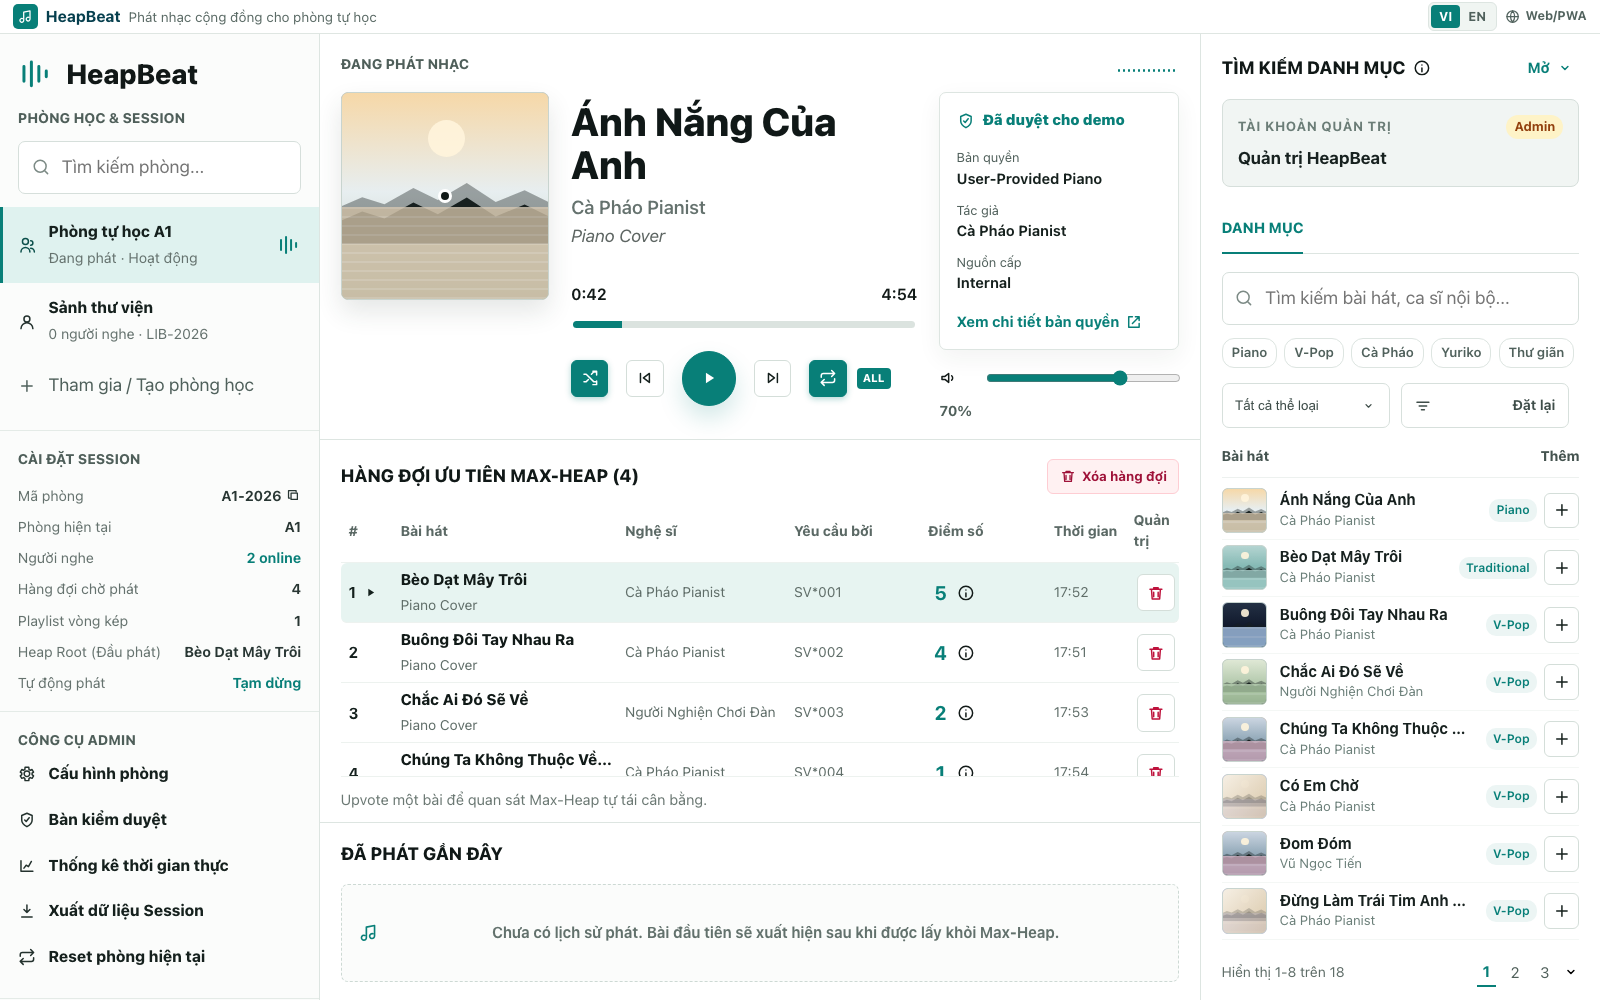
\includegraphics[width=0.97\textwidth]{screenshot-desktop.png}}
\caption{Giao diện HeapBeat tại 1600x1000 với danh mục piano và Max-Heap gồm 4 phần tử.}
\end{figure}

\begin{table}[h]\centering\small
\begin{tabularx}{\textwidth}{@{}p{2.6cm}Xp{3.9cm}@{}}
\toprule
\textbf{Bề mặt} & \textbf{Kết quả hiện thực} & \textbf{CTDL/logic quan sát được}\\
\midrule
Trình phát & Phát/tạm dừng, Next/Prev, tua, âm lượng, các chế độ lặp và thông tin ghi công. &
Con trỏ \code{current/next/prev} của CDLL\\
Hàng đợi ưu tiên & Làm nổi bật gốc Heap, điểm, thời điểm, bình chọn và thao tác xóa; thứ tự
đổi ngay sau khi bình chọn. & Max-Heap + Map chỉ số\\
Danh mục bài hát & Tìm kiếm, lọc thể loại, phân trang và chỉ cho phép yêu cầu bài hợp lệ. &
Kiểm tra giấy phép + thêm vào Heap\\
Kiểm duyệt & Duyệt hoặc từ chối giấy phép, xem tài khoản bị chặn và bỏ chặn thủ công. &
SpamGuard Hash Map\\
Phòng và thống kê & Tạo hoặc chuyển phòng độc lập, theo dõi kết nối và thống kê điểm,
lịch sử, vi phạm. & Trạng thái phòng + nhật ký\\
\bottomrule
\end{tabularx}
\end{table}

Ngoài ba yêu cầu cấu trúc dữ liệu cốt lõi, sản phẩm còn hỗ trợ phân quyền sinh viên/quản trị
viên, xuất phiên làm việc dưới dạng JSON, giao diện song ngữ, phím tắt điều khiển, lưu trạng
thái phiên, kiểm duyệt giấy phép và đồng bộ tùy chọn trong mạng nội bộ.

\newpage

% PAGE 8 -----------------------------------------------------------------------
\chapter{Kiểm thử và kết quả}
\section{Thiết kế kiểm tra và tiêu chí đánh giá}
Mỗi phép kiểm tra bắt đầu từ một trạng thái dữ liệu xác định. Các kiểm thử đơn vị gọi trực
tiếp lớp cấu trúc dữ liệu; chương trình C sử dụng \code{assert}; bản dựng TypeScript được
kiểm tra kiểu tĩnh trước khi đóng gói. Một trường hợp chỉ được công nhận khi cả kết quả trả
về lẫn bất biến sau thao tác đều đúng. Đối với giao diện thích ứng, điều kiện chấp nhận là
\code{scrollWidth = clientWidth} cho thân trang và vùng hàng đợi, nội dung chính không bị
cắt và các điều khiển vẫn có nhãn hỗ trợ truy cập.

\begin{table}[h]\centering\small
\begin{tabularx}{\textwidth}{@{}p{3cm}p{4.2cm}X@{}}
\toprule
\textbf{Thành phần} & \textbf{Môi trường/lệnh} & \textbf{Điều kiện kiểm chứng}\\
\midrule
TypeScript CTDL & Node.js 20+, Vitest; \code{npm run test} & Giá trị trả về, thứ tự gốc Heap,
liên kết vòng và trạng thái SpamGuard\\
Mã đối chiếu C & C11, \code{-Wall -Wextra -Werror} & Tất cả \code{assert} đạt, không cảnh báo biên dịch\\
Bản dựng ứng dụng & TypeScript + Vite; \code{npm run build} & Hoàn tất bản dựng, 38 module được xử lý\\
Giao diện thích ứng & Trình duyệt hiện đại; 1400x900, 1200x820, 390x844 & Không tràn thân
trang hoặc hàng đợi; bảng thu gọn cột và chuyển thành thẻ ở kích thước điện thoại\\
\bottomrule
\end{tabularx}
\caption{Môi trường đánh giá và tiêu chí xác nhận kết quả.}
\label{tab:experiment}
\end{table}

\section{Kiểm thử đơn vị cho cấu trúc dữ liệu}
Lệnh \code{npm run test} thực hiện 22 phép kiểm tra bằng Vitest. Các phép kiểm tra tác động
trực tiếp lên lớp cấu trúc dữ liệu, trạng thái phát và danh mục MP3, không phụ thuộc vào ảnh
chụp màn hình hoặc thao tác thủ công.

\begin{table}[h]\centering\small
\begin{tabularx}{\textwidth}{@{}p{2.7cm}Xp{2.4cm}@{}}
\toprule
\textbf{Nhóm} & \textbf{Ca kiểm thử tiêu biểu} & \textbf{Kết quả}\\
\midrule
Circular DLL (4) & Danh sách rỗng; vòng tail$\to$head; vòng head$\to$tail; addLast không phá liên kết. &
\status{4/4 đạt}\\
Max-Heap (7) & Gốc có ưu tiên cao nhất; heapify hai hướng; thứ tự FIFO khi bằng điểm; lấy,
xóa và gỡ bình chọn của người bị chặn. &
\status{7/7 đạt}\\
SpamGuard (5) & Cho phép 3 yêu cầu; chặn yêu cầu thứ tư; phát hiện bài trùng; thu hồi bài;
loại mốc cũ và hết thời hạn chặn. &
\status{5/5 đạt}\\
Trạng thái phát (4) & Phòng rỗng; xóa hàng đợi; từ chối bài đang phát; sửa vị trí phát lưu sai. &
\status{4/4 đạt}\\
Danh mục MP3 (2) & Đủ 18 file, ID và đường dẫn không trùng; URL hoạt động khi triển khai
trong thư mục con. &
\status{2/2 đạt}\\
\bottomrule
\end{tabularx}
\end{table}

\section{Tạo bản dựng và kiểm tra tích hợp trên trình duyệt}
\begin{itemize}
  \item \code{npm run format:check}: toàn bộ TypeScript, CSS và script đúng định dạng.
  \item \code{npm run build}: TypeScript và Vite tạo bản dựng hoàn chỉnh; 38 module được xử lý.
  \item Bộ kiểm thử C: chạy \code{make test} trong thư mục \code{backend-c};
  GCC/Clang dùng \code{-Wall -Wextra -Werror} và cả 56 assertion đều đạt.
  \item Trình duyệt: tiêu đề và URL đúng; trang hiển thị đầy đủ; không có lỗi hoặc cảnh báo
  trên console liên quan đến ứng dụng.
  \item Các tình huống đã thực hiện gồm: quản trị viên đăng nhập; Next lấy gốc Heap làm hàng
  đợi giảm từ 4 xuống 3; Prev quay lại đúng node trong CDLL; duyệt giấy phép làm nút yêu cầu
  khả dụng; bình chọn làm điểm tăng từ 4 lên 5 và thay đổi gốc Heap; tài khoản SV9999 gửi
  trùng bị chặn và các bài liên quan được thu hồi; phòng mới hoạt động độc lập; giao diện
  chuyển đúng sang bố cục điện thoại.
\end{itemize}

Tại kích thước máy tính hẹp 1200x820, cột giữa rộng 660 px và hàng đợi có
\code{clientWidth = scrollWidth = 591 px}; ở mobile 390x844, body có
\code{clientWidth = scrollWidth = 375 px} và hàng đợi có
\code{clientWidth = scrollWidth = 345 px}. Đây là bằng chứng đo trực tiếp cho việc loại
bỏ cuộn ngang từng xuất hiện ở bảng 7 cột. Ở mức hẹp, nghệ sĩ và thời gian được đưa vào
dòng thông tin phụ của bài; ở điện thoại, mỗi yêu cầu chuyển thành thẻ hai hàng nhưng vẫn
giữ thứ hạng, người yêu cầu, điểm và thao tác quản trị.

Các trường hợp biên cũng được đưa vào bộ kiểm thử: xóa hết hàng đợi không làm mất bài đang
phát; danh sách phát rỗng luôn đưa vị trí phát về \code{null/0}; và dữ liệu danh mục cũ
không thể ghi đè danh mục piano sau khi nâng cấp.

\begin{figure}[h]
\centering
\begin{minipage}[t]{0.46\textwidth}\centering
\setlength{\fboxsep}{2pt}%
\fcolorbox{hbline}{white}{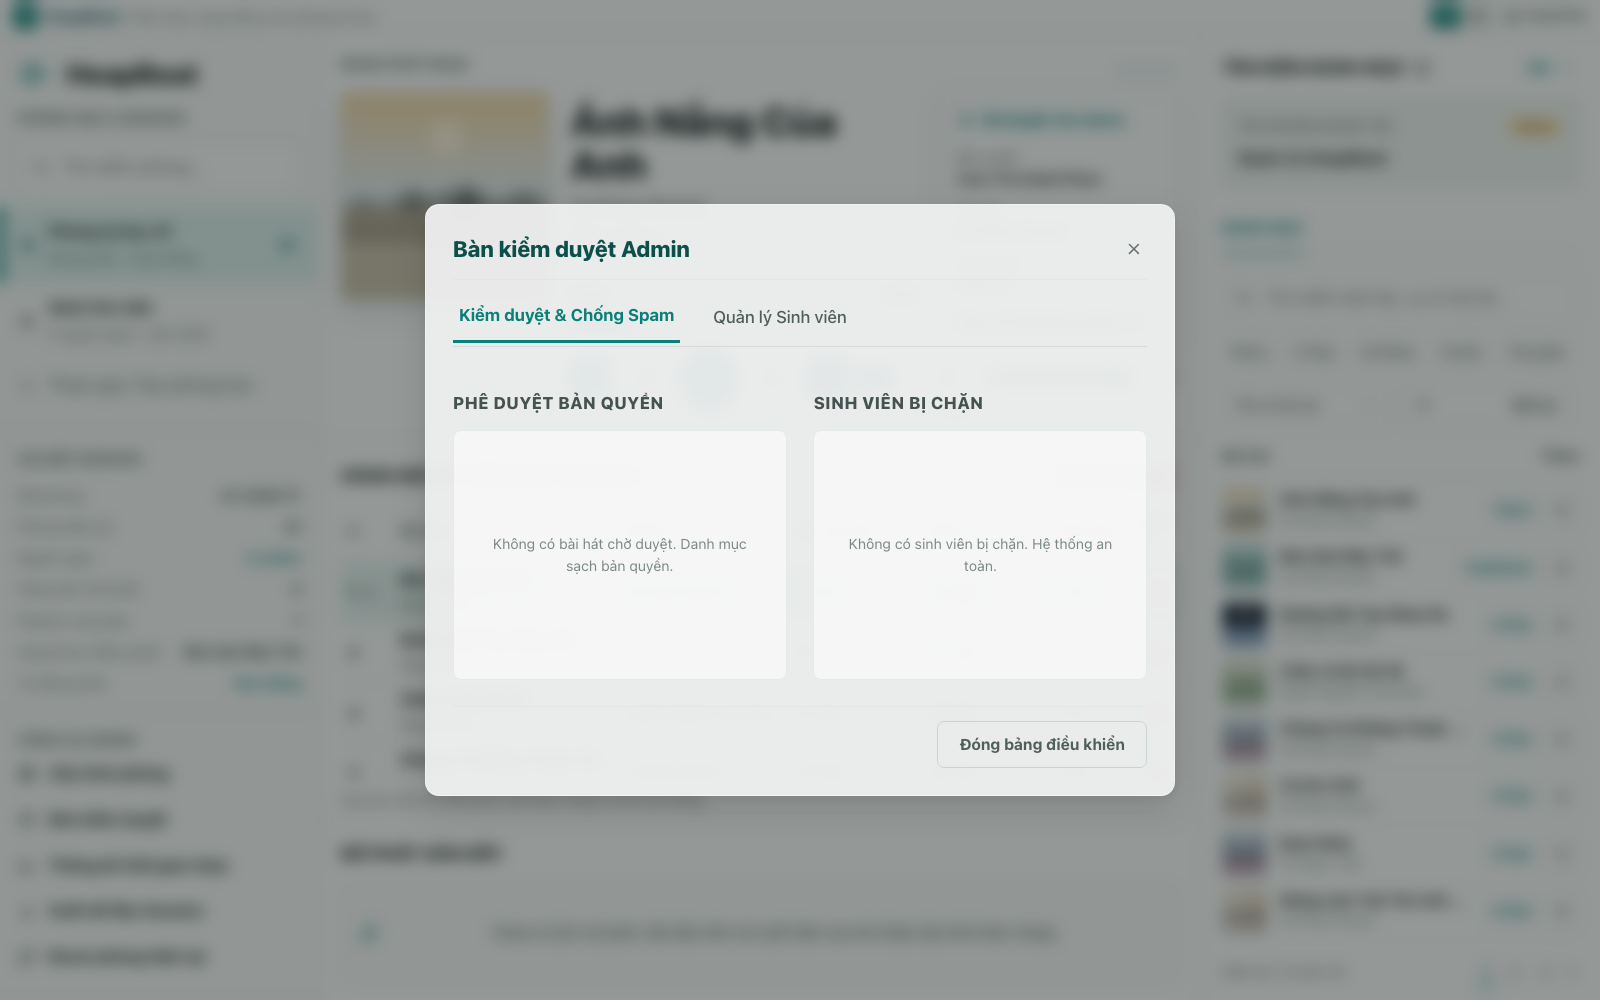
\includegraphics[width=\dimexpr\linewidth-2\fboxsep-2\fboxrule\relax]{screenshot-moderation.png}}\par
\vspace{3pt}{\footnotesize\textbf{Bàn kiểm duyệt:} danh mục đã duyệt và không có tài khoản bị chặn.\par}
\end{minipage}\hfill
\begin{minipage}[t]{0.32\textwidth}\centering
\setlength{\fboxsep}{2pt}%
\fcolorbox{hbline}{white}{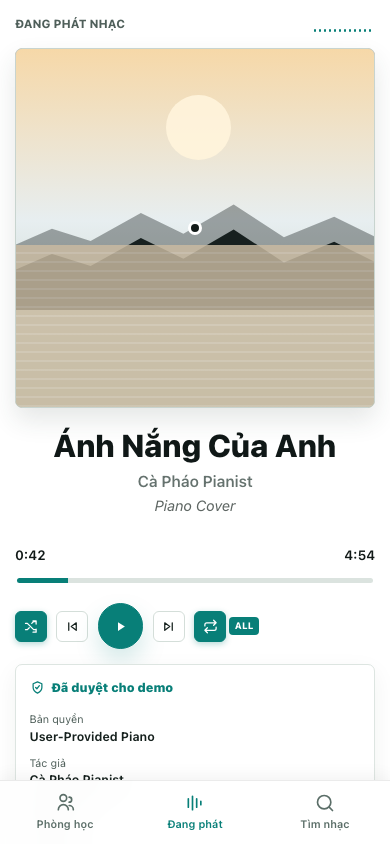
\includegraphics[height=4.8cm]{screenshot-mobile.png}}\par
\vspace{3pt}{\footnotesize\textbf{Điện thoại 390x844:} trình phát không tràn ngang.\par}
\end{minipage}
\end{figure}

% PAGE 9 -----------------------------------------------------------------------
\clearpage
\chapter{Phân tích và đánh giá}
\section{Trả lời câu hỏi nghiên cứu}
\begin{table}[h]\centering\small
\begin{tabularx}{\textwidth}{@{}p{1cm}p{5.1cm}X@{}}
\toprule
\textbf{RQ} & \textbf{Kết quả kiểm tra} & \textbf{Kết luận trong phạm vi đề tài}\\
\midrule
RQ1 & 7/7 phép kiểm tra Heap; bộ so sánh và Map chỉ số được kiểm tra sau thao tác thêm,
bình chọn, xóa và lấy gốc. & Max-Heap giữ đúng phần tử gốc, quy tắc phân giải khi bằng điểm
và chi phí cập nhật $O(\log n)$.\\
RQ2 & 4/4 phép kiểm tra CDLL cho danh sách rỗng, một node và khép vòng hai chiều. &
Next/Prev/Repeat có chi phí $O(1)$ và không cần xử lý chỉ số biên.\\
RQ3 & 5/5 phép kiểm tra SpamGuard cùng phép kiểm tra thu hồi khỏi Heap. & Tra cứu trung
bình $O(1)$, phát hiện yêu cầu trùng hoặc vượt giới hạn và trả đúng các ID cần thu hồi.\\
\bottomrule
\end{tabularx}
\caption{Kết quả trả lời ba câu hỏi nghiên cứu.}
\label{tab:rq-results}
\end{table}

\section{So sánh lựa chọn hàng đợi ưu tiên}
\begin{table}[h]\centering\small
\begin{tabularx}{\textwidth}{@{}lcccX@{}}
\toprule
\textbf{Phương án} & \textbf{Xem cực đại} & \textbf{Thêm} & \textbf{Đổi bình chọn} & \textbf{Đánh giá}\\
\midrule
Mảng chưa sắp xếp & $O(n)$ & $O(1)$ & $O(1)$ & Khi phát bài phải quét toàn bộ mảng.\\
Mảng luôn sắp xếp & $O(1)$ & $O(n)$ & $O(n)$ & Bình chọn liên tục làm dịch chuyển nhiều phần tử.\\
Cây cân bằng & $O(\log n)$ & $O(\log n)$ & $O(\log n)$ & Đáp ứng yêu cầu nhưng làm phần hiện thực phức tạp hơn.\\
\textbf{Max-Heap + Map} & \textbf{$O(1)$} & \textbf{$O(\log n)$} & \textbf{$O(\log n)$} &
Cân bằng giữa hiệu năng, bộ nhớ và khả năng minh họa.\\
\bottomrule
\end{tabularx}
\end{table}

\section{Điểm mạnh}
\begin{itemize}
  \item Ba cấu trúc dữ liệu tương ứng rõ với ba yêu cầu cốt lõi; lớp thuật toán không phụ
  thuộc vào React nên có thể kiểm tra riêng.
  \item Map chỉ số giúp thay đổi bình chọn mà không phải quét tìm yêu cầu; quy tắc phân giải
  khi bằng điểm được xác định và giữ ổn định.
  \item SpamGuard không chỉ từ chối yêu cầu mới mà còn trả về các ID để thu hồi toàn bộ bài
  đang chờ của tài khoản vi phạm.
  \item Giao diện lọc theo hồ sơ giấy phép; backend C chỉ nhận mã bài thuộc danh mục cố định;
  18 file piano đều có thông tin ghi công và mô tả phạm vi sử dụng.
  \item Giao diện thể hiện rõ gốc Heap, điểm số và vòng lịch sử phát, tạo điều kiện đối chiếu
  giữa lý thuyết và hành vi chương trình.
\end{itemize}

\section{Hạn chế và rủi ro còn lại}
\begin{itemize}
  \item Backend C hiện lưu state trong RAM; cần bổ sung cơ sở dữ liệu và cơ chế phục hồi
  khi triển khai lâu dài hoặc vận hành nhiều phòng.
  \item Tài khoản minh họa được lưu ở phía trình duyệt; hệ thống chưa có SSO, băm mật khẩu
  tại máy chủ, token, giới hạn theo IP hoặc kiểm soát quyền ở máy chủ.
  \item Số người nghe hiện được ước lượng bằng số tab gửi tín hiệu định kỳ, không phải số
  người dùng duy nhất đã xác thực.
  \item Chưa đo tải với hàng nghìn yêu cầu và chưa kiểm thử PWA trên nhiều thiết bị thật.
  \item Quyền biểu diễn công cộng phụ thuộc địa điểm và giấy phép cụ thể; phần mềm không
  thể tự suy ra quyền pháp lý chỉ từ một URL.
\end{itemize}

\section{Mối đe dọa đến độ tin cậy}
\begin{itemize}
  \item \textbf{Độ tin cậy nội tại:} bộ kiểm thử được xây dựng từ cùng đặc tả với chương
  trình nên có thể lặp lại một giả định sai. Chương trình C độc lập và việc kiểm tra trên
  giao diện làm giảm nhưng không loại bỏ hoàn toàn rủi ro này.
  \item \textbf{Khả năng khái quát:} dữ liệu chỉ gồm 18 bài và hàng đợi nhỏ; chưa thể suy ra
  độ trễ khi có hàng nghìn yêu cầu hoặc nhiều phòng cập nhật đồng thời.
  \item \textbf{Độ tin cậy đo lường:} số người nghe hiện được suy ra từ tín hiệu của tab;
  phép đo kích thước DOM chưa thay thế đánh giá khả dụng với người dùng thật.
  \item \textbf{Độ tin cậy pháp lý:} metadata và URL giấy phép là bằng chứng kỹ thuật,
  không tự động xác lập quyền biểu diễn công cộng tại mọi địa điểm.
\end{itemize}

% PAGE 10 ----------------------------------------------------------------------
\clearpage
\chapter{Kết luận và hướng phát triển}
Kết quả cho thấy bản nộp HeapBeat đáp ứng các yêu cầu đã đặt ra. Max-Heap đưa bài có mức ưu
tiên cao nhất lên đầu hàng đợi; danh sách liên kết đôi vòng hỗ trợ Next/Prev/Repeat; Hash
Map kiểm soát tần suất gửi yêu cầu theo StudentID. Các thao tác chính có chi phí
$O(\log n)$ hoặc $O(1)$ trung bình. Nhận định này được đối chiếu bằng 22 kiểm thử đơn vị,
chương trình C, bản dựng web và các tình huống sử dụng trên máy tính lẫn điện thoại.

\section{Hướng phát triển ưu tiên}
\begin{enumerate}
  \item Chuyển trạng thái sang PostgreSQL/Redis và WebSocket để nhiều thiết bị cập nhật đồng thời.
  \item Tích hợp SSO của trường, xác thực tại máy chủ, RBAC, băm mật khẩu và nhật ký bất biến.
  \item Bổ sung nhập dữ liệu từ Openverse/Jamendo theo quy trình tìm kiếm, chờ duyệt và lưu
  hồ sơ; không tự động phát ngay sau khi nhập.
  \item Kiểm thử PWA trên Windows, macOS, Android và iOS; bổ sung icon PNG cho từng thiết bị.
  \item Bổ sung cơ chế giảm trọng số bình chọn theo thời gian, phát hiện thông đồng và đo Heap với dữ liệu lớn.
\end{enumerate}

\cleardoublepage
\phantomsection
\addcontentsline{toc}{chapter}{Tài liệu tham khảo}
{\small
\begin{thebibliography}{9}
\bibitem{cormen2022}
T. H. Cormen, C. E. Leiserson, R. L. Rivest, and C. Stein,
\textit{Introduction to Algorithms}, 4th ed. MIT Press, 2022.

\bibitem{sedgewick2011}
R. Sedgewick and K. Wayne, \textit{Algorithms}, 4th ed. Addison-Wesley, 2011.

\bibitem{reactdocs}
React Team, ``React Documentation.'' \url{https://react.dev/} (truy cập 04/08/2026).

\bibitem{vitedocs}
Vite Team, ``Vite Guide.'' \url{https://vite.dev/guide/} (truy cập 04/08/2026).

\bibitem{mdnaudio}
MDN Web Docs, ``HTMLAudioElement.''
\url{https://developer.mozilla.org/docs/Web/API/HTMLAudioElement} (truy cập 04/08/2026).

\bibitem{cclicenses}
Creative Commons, ``About CC Licenses.''
\url{https://creativecommons.org/share-your-work/cclicenses/} (truy cập 04/08/2026).

\bibitem{openverse}
Openverse, ``Openverse API Documentation.'' \url{https://api.openverse.org/}
(truy cập 04/08/2026).

\bibitem{spotify}
Spotify, ``Developer Policy.'' \url{https://developer.spotify.com/policy}
(truy cập 04/08/2026).
\end{thebibliography}
}

\cleardoublepage
\appendix
\chapter{Các thuật toán trọng tâm và giải thích từng dòng}
\pagelead{Phụ lục sử dụng mã giả rút gọn, tương đương với phần hiện thực trong backend C11.
Tên hàm, thứ tự kiểm tra và bất biến
được giữ nguyên; các bước sao chép dữ liệu và tạo phản hồi giao diện không ảnh hưởng đến
thuật toán được lược bỏ.}

\begin{table}[H]\centering\footnotesize
\begin{tabularx}{\textwidth}{@{}p{1cm}p{4.15cm}p{4.1cm}Xp{2.2cm}@{}}
\toprule
\textbf{ID} & \textbf{Thuật toán} & \textbf{Mục đích} & \textbf{Độ phức tạp} &
\textbf{Kết quả đối chiếu}\\
\midrule
A1 & Bộ so sánh đa tiêu chí & Xác định thứ tự toàn phần cho hàng đợi & $O(1)$ & 7 phép kiểm tra Heap\\
A2 & Insert + heapifyUp & Thêm yêu cầu và đưa phần tử ưu tiên lên trên & $O(\log n)$ & Thêm/tăng điểm\\
A3 & ChangeVote & Đổi bình chọn, tính lại điểm và chọn hướng heapify & $O(\log n)$ & Chuyển trạng thái bình chọn\\
A4 & ExtractMax & Lấy gốc Heap làm bài kế tiếp & $O(\log n)$ & Lấy gốc Heap\\
A5 & Remove tùy ý & Xóa yêu cầu giữa Heap, giữ đúng Map chỉ số & $O(\log n)$ & Xóa/thu hồi\\
A6 & CDLL add/next/prev & Quản lý lịch sử và lặp toàn bộ & Add/Next/Prev $O(1)$ & 4 phép kiểm tra CDLL\\
A7 & Kiểm tra và chặn & Cửa sổ trượt, bài trùng, hạn mức và thu hồi & TB $O(1)+O(r)$ & 5 phép kiểm tra SpamGuard\\
A8 & Chuyển bài & Phối hợp Heap với CDLL theo chế độ lặp & $O(\log n)$ hoặc $O(1)$ & Kiểm tra trạng thái phát\\
\bottomrule
\end{tabularx}
\caption{Danh mục thuật toán được phân tích chi tiết.}
\label{tab:algorithm-catalog}
\end{table}

\Needspace{12\baselineskip}
\section{Bộ so sánh đa tiêu chí}
\begin{lstlisting}[style=algorithm]
compare(a, b):                              // [D1] negative means a ranks first
  if a.score != b.score:                   // [D2] score is the primary key
    return b.score - a.score               // [D3] descending score
  if a.upvotes != b.upvotes:               // [D4] use upvotes when scores tie
    return b.upvotes - a.upvotes           // [D5] descending upvotes
  aTie = a.shuffleOrder ?? INFINITY        // [D6] unshuffled items rank later
  bTie = b.shuffleOrder ?? INFINITY        // [D7] same rule for b
  if aTie != bTie:                         // [D8] compare only when different
    return aTie - bTie                     // [D9] smaller shuffle order first
  return a.requestedAt - b.requestedAt     // [D10] final FIFO tie-break
\end{lstlisting}
\begin{description}[leftmargin=1.2cm,labelwidth=0.8cm,style=multiline,
  font=\ttfamily\bfseries,itemsep=2pt]
  \item[D1] Khai báo bộ so sánh; giá trị âm nghĩa là \code{a} có ưu tiên cao hơn \code{b}.
  \item[D2] Điểm là khóa chính; chỉ xét các tiêu chí phụ khi hai điểm bằng nhau.
  \item[D3] Trả chênh lệch theo thứ tự giảm dần, nên điểm lớn đứng trước.
  \item[D4] Nếu bằng điểm, số lượt tăng bình chọn là khóa thứ hai để ưu tiên mức đồng thuận dương.
  \item[D5] Phần tử có nhiều lượt tăng bình chọn hơn tiếp tục đứng trước.
  \item[D6] Yêu cầu chưa được xáo thứ tự nhận giá trị vô cực, nên không chen trước thứ tự
  do quản trị viên đã gán.
  \item[D7] Áp dụng cùng quy ước cho phần tử \code{b}.
  \item[D8] Chỉ xét thứ tự xáo khi hai giá trị thực sự khác nhau.
  \item[D9] Số thứ tự xáo nhỏ hơn có ưu tiên cao hơn.
  \item[D10] Cuối cùng dùng thời điểm tăng dần để bảo đảm FIFO và kết quả xác định.
\end{description}
\textbf{Bất biến:} bộ so sánh tạo thứ tự nhất quán theo bộ
$(\text{điểm}\downarrow,\text{lượt tăng}\downarrow,shuffleOrder\uparrow,requestedAt\uparrow)$.
Mọi hàm xếp hạng và Heap phải dùng cùng bộ so sánh để giao diện không hiển thị khác gốc Heap.

\Needspace{12\baselineskip}
\section{Thêm phần tử và \code{heapifyUp}}
\begin{lstlisting}[style=algorithm]
insert(item):                               // [D1] receive a valid request
  heap.push(clone(item))                    // [D2] isolate external references
  indexMap[item.id] = heap.length - 1       // [D3] record O(1) lookup position
  i = heap.length - 1                      // [D4] start at the new leaf
  while i > 0:                             // [D5] stop at the root
    p = floor((i - 1) / 2)                 // [D6] compute parent index
    if not higherPriority(heap[i], heap[p]): // [D7] invariant already holds
      break                                // [D8] terminate early
    swap(heap[i], heap[p])                  // [D9] move item up one level
    indexMap[heap[i].id] = i               // [D10] fix descending item index
    indexMap[heap[p].id] = p               // [D11] fix ascending item index
    i = p                                  // [D12] continue from parent
\end{lstlisting}
\begin{description}[leftmargin=1.2cm,labelwidth=0.8cm,style=multiline,
  font=\ttfamily\bfseries,itemsep=2pt]
  \item[D1] Nhận một yêu cầu đã có ID duy nhất và điểm đã được tính.
  \item[D2] Sao chép trước khi lưu để bên gọi không thể sửa ngầm phần tử trong Heap.
  \item[D3] Ghi vị trí mới vào Hash Map chỉ số, cho phép tìm yêu cầu trong $O(1)$ trung bình.
  \item[D4] Bắt đầu tại lá vừa thêm ở cuối mảng.
  \item[D5] Gốc không có cha; vòng lặp dừng khi \code{i=0}.
  \item[D6] Tính vị trí cha trong biểu diễn mảng của cây nhị phân.
  \item[D7] Nếu con không ưu tiên hơn cha thì bất biến đã đúng trên toàn đường đi.
  \item[D8] Dừng sớm, tránh các phép so sánh không cần thiết.
  \item[D9] Đổi con với cha để đưa phần tử ưu tiên cao lên một mức.
  \item[D10] Sau khi đổi chỗ, cập nhật vị trí phần tử vừa đi xuống.
  \item[D11] Cập nhật vị trí phần tử vừa đi lên; thiếu hai dòng này làm Map chỉ số sai.
  \item[D12] Tiếp tục kiểm tra từ vị trí cha cũ cho đến gốc hoặc điểm ổn định.
\end{description}
\textbf{Đúng đắn:} trước khi thêm, Heap hợp lệ. Chỉ đường từ lá mới đến gốc có thể vi phạm;
mỗi lần đổi chỗ sửa một cạnh vi phạm và không phá các cây con. Chiều cao Heap là
$\lfloor\log_2 n\rfloor$, nên thời gian $O(\log n)$, bộ nhớ phụ $O(1)$.

\Needspace{12\baselineskip}
\section{Thay đổi bình chọn và chọn hướng tái cân bằng}
\begin{lstlisting}[style=algorithm]
changeVote(requestId, studentId, nextVote): // [D1] target vote is -1, 0, or 1
  i = indexMap.get(requestId)               // [D2] avoid a linear scan
  if i is missing: return null              // [D3] request already left queue
  oldVote = heap[i].votes[studentId] ?? 0   // [D4] absent vote equals zero
  if oldVote == nextVote: return delta 0    // [D5] idempotent transition
  votes = clone(heap[i].votes)              // [D6] preserve input state
  if nextVote == 0: delete votes[studentId] // [D7] zero removes the key
  else: votes[studentId] = nextVote         // [D8] store upvote/downvote
  updated = rebuildItem(heap[i], votes)     // [D9] rebuild score from snapshot
  delta = nextVote - oldVote                // [D10] supports direct switches
  heap[i] = updated                         // [D11] replace at current index
  if delta > 0: heapifyUp(i)                // [D12] score increased: move up
  else: heapifyDown(i)                      // [D13] score decreased: move down
  j = indexMap.get(requestId)               // [D14] reread index after heapify
  return clone(heap[j]), delta              // [D15] return command result
\end{lstlisting}
\begin{description}[leftmargin=1.2cm,labelwidth=0.8cm,style=multiline,
  font=\ttfamily\bfseries,itemsep=2pt]
  \item[D1] Hàm nhận yêu cầu, người bình chọn và trạng thái đích thuộc tập $\{-1,0,1\}$.
  \item[D2] Map chỉ số loại bỏ bước quét tuyến tính qua hàng đợi.
  \item[D3] Yêu cầu có thể đã được lấy hoặc xóa; trả \code{null} giúp API phản hồi an toàn.
  \item[D4] Bình chọn chưa tồn tại được xem là 0.
  \item[D5] Bình chọn cùng chiều lần hai là thao tác lặp an toàn; điểm không đổi.
  \item[D6] Sao chép bản đồ bình chọn để không sửa trạng thái đầu vào.
  \item[D7] Trạng thái 0 được biểu diễn bằng việc xóa khóa, làm gọn ảnh chụp trạng thái.
  \item[D8] Hai trạng thái còn lại được lưu trực tiếp.
  \item[D9] Tính lại số lượt tăng, lượt giảm và điểm từ toàn bộ bình chọn thay vì cộng dồn dễ sai.
  \item[D10] Delta đúng cả chuyển trực tiếp $1\to-1$ ($-2$) và $-1\to1$ ($+2$).
  \item[D11] Thay phần tử tại đúng chỉ số nhưng chưa đổi cấu trúc cây.
  \item[D12] Độ lệch dương chỉ có thể vi phạm với cha, nên tái cân bằng lên trên.
  \item[D13] Độ lệch âm chỉ có thể vi phạm với con, nên tái cân bằng xuống dưới.
  \item[D14] Quá trình tái cân bằng có thể đổi chỉ số; phải đọc lại vị trí từ Map.
  \item[D15] Trả bản sao phần tử ở vị trí mới cùng độ lệch để dịch vụ tạo phản hồi JSON.
\end{description}
\textbf{Độ phức tạp:} tìm chỉ số trong $O(1)$ trung bình, tái tạo bình chọn $O(v)$ với $v$
là số người đã bình chọn yêu cầu, và tái cân bằng $O(\log n)$. Trong mô hình lớp học, $v$
bị chặn bởi số tài khoản;
phần thay đổi cấu trúc Heap vẫn là $O(\log n)$.

\Needspace{12\baselineskip}
\section{ExtractMax}
\begin{lstlisting}[style=algorithm]
extractMax():                               // [D1] remove highest-priority item
  if heap.length == 0: return null          // [D2] guard an empty Heap
  max = heap[0]                             // [D3] root is the next track
  last = heap.pop()                         // [D4] keep the array contiguous
  indexMap.delete(max.id)                   // [D5] delete stale mapping
  if heap.length > 0:                       // [D6] restore if items remain
    heap[0] = last                          // [D7] fill the root hole
    indexMap[last.id] = 0                   // [D8] fix index before heapify
    heapifyDown(0)                          // [D9] restore downward
  return clone(max)                         // [D10] hide internal reference
\end{lstlisting}
\begin{description}[leftmargin=1.2cm,labelwidth=0.8cm,style=multiline,
  font=\ttfamily\bfseries,itemsep=2pt]
  \item[D1] Lấy và xóa phần tử ưu tiên cao nhất.
  \item[D2] Heap rỗng trả null; không truy cập index 0 ngoài miền.
  \item[D3] Bất biến Heap bảo đảm phần tử gốc chính là bài cần phát.
  \item[D4] Lấy phần tử cuối để giữ mảng liên tục.
  \item[D5] Yêu cầu đã rời Heap nên phải xóa khỏi Map chỉ số.
  \item[D6] Nếu phần tử vừa lấy là phần tử duy nhất thì không cần khôi phục cây.
  \item[D7] Đặt lá cuối vào vị trí trống ở gốc.
  \item[D8] Ghi lại chỉ số 0 trước khi tái cân bằng.
  \item[D9] Gốc mới chỉ có thể vi phạm với con, vì vậy dùng \code{heapifyDown}.
  \item[D10] Trả bản sao để tầng HTTP không giữ tham chiếu nội bộ.
\end{description}
\textbf{Độ phức tạp:} $O(\log n)$ thời gian và $O(1)$ bộ nhớ phụ. Peek riêng lẻ vẫn
$O(1)$; extract phải trả lại bất biến sau khi xóa.

\Needspace{12\baselineskip}
\section{Xóa một yêu cầu bất kỳ}
\begin{lstlisting}[style=algorithm]
remove(requestId):                          // [D1] admin remove or spam purge
  i = indexMap.get(requestId)               // [D2] average O(1) lookup
  if i is missing: return null              // [D3] repeated delete is safe
  removed = heap[i]                         // [D4] retain record for audit
  last = heap.pop()                         // [D5] take leaf to fill the hole
  indexMap.delete(requestId)                // [D6] remove stale mapping
  if i < heap.length:                       // [D7] skip if last was removed
    heap[i] = last                          // [D8] fill the vacant index
    indexMap[last.id] = i                   // [D9] synchronize the Map
    heapifyUp(i)                            // [D10] test violation with parent
    j = indexMap.get(last.id)               // [D11] reread the new index
    heapifyDown(j)                          // [D12] test violation with child
  return clone(removed)                     // [D13] return removed request
\end{lstlisting}
\begin{description}[leftmargin=1.2cm,labelwidth=0.8cm,style=multiline,
  font=\ttfamily\bfseries,itemsep=2pt]
  \item[D1] Xóa theo ID yêu cầu, dùng khi quản trị viên xóa hoặc SpamGuard thu hồi.
  \item[D2] Tra vị trí trung bình $O(1)$ bằng Map.
  \item[D3] Bảo đảm thao tác lặp lại vẫn an toàn khi yêu cầu đã biến mất.
  \item[D4] Giữ phần tử bị xóa để ghi nhật ký.
  \item[D5] Lấy phần tử cuối nhằm lấp lỗ mà không dịch mảng $O(n)$.
  \item[D6] Xóa ánh xạ của phần tử không còn tồn tại.
  \item[D7] Nếu xóa đúng phần tử cuối, thao tác lấy cuối đã hoàn tất việc xóa.
  \item[D8] Đưa phần tử cuối vào vị trí trống.
  \item[D9] Đồng bộ Map ngay sau khi thay vị trí.
  \item[D10] Ưu tiên mới có thể lớn hơn cha, nên thử \code{heapifyUp} trước.
  \item[D11] Đọc lại chỉ số vì phần tử có thể đã đi lên.
  \item[D12] Từ vị trí mới, thử \code{heapifyDown} để bao phủ trường hợp nhỏ hơn con.
  \item[D13] Trả bản sao yêu cầu đã xóa.
\end{description}
\textbf{Lý do chạy hai hướng:} phần tử cuối thay thế một vị trí bất kỳ, nên chưa biết nó
vi phạm với cha hay với con. Sau \code{heapifyUp}, đọc lại chỉ số rồi dùng \code{heapifyDown}
bảo đảm đúng cả
hai trường hợp mà vẫn $O(\log n)$.

\Needspace{12\baselineskip}
\section{Danh sách liên kết đôi vòng}
\begin{lstlisting}[style=algorithm]
addLast(value):                              // [D1] append track to history
  node = new Node(value)                    // [D2] allocate a new node
  if head == null:                          // [D3] list is empty
    node.prev = node; node.next = node      // [D4] valid one-node ring
    head = node; current = node             // [D5] initialize head/current
  else:                                     // [D6] list is non-empty
    tail = head.prev                        // [D7] get tail in O(1)
    tail.next = node; node.prev = tail      // [D8] link to old tail
    node.next = head; head.prev = node      // [D9] close ring with head
  length = length + 1                       // [D10] increment after linking

next(): if current != null: current = current.next // [D12] advance and wrap
prev(): if current != null: current = current.prev // [D13] rewind and wrap
\end{lstlisting}
\begin{description}[leftmargin=1.2cm,labelwidth=0.8cm,style=multiline,
  font=\ttfamily\bfseries,itemsep=2pt]
  \item[D1] Nối một bài đã phát vào cuối lịch sử.
  \item[D2] Cấp phát nút mới; chỉ số của nút bằng độ dài trước khi tăng.
  \item[D3] Tách trường hợp rỗng vì chưa có nút cuối.
  \item[D4] Một nút tự trỏ cả hai chiều, tạo vòng hợp lệ có kích thước một.
  \item[D5] Nút đầu và nút hiện hành cùng trỏ đến phần tử đầu tiên.
  \item[D6] Nhánh danh sách không rỗng.
  \item[D7] Trong CDLL, nút cuối luôn là \code{head.prev}, truy cập trong $O(1)$.
  \item[D8] Nối nút cuối cũ sang nút mới và nút mới lùi về nút cuối cũ.
  \item[D9] Khép vòng: nút mới tiến về nút đầu, còn nút đầu lùi về nút mới.
  \item[D10] Tăng kích thước sau khi bốn liên kết đã nhất quán.
  \item[D12] Next chỉ đổi một con trỏ; tại nút cuối, \code{next=head} tạo chế độ lặp toàn bộ tự nhiên.
  \item[D13] Previous hoạt động đối xứng; tại nút đầu, \code{prev=tail}.
\end{description}
\textbf{Bất biến:} với mọi nút $x$,
\code{x.next.prev=x} và \code{x.prev.next=x}; \code{head.prev} là tail và
\code{tail.next} là head. AddLast, Next và Prev đều $O(1)$.

\Needspace{12\baselineskip}
\section{Cửa sổ trượt, chặn và thu hồi}
\begin{lstlisting}[style=algorithm]
checkBeforeRequest(student, song, now):       // [D1] run before touching Heap
  state = getOrCreate(student)               // [D2] get/create StudentID state
  state.recent = filter(t >= now - WINDOW)   // [D3] prune outside 10 minutes
  if state.blockedUntil > now:               // [D4] prioritize active block
    return BLOCKED with no new purge         // [D5] avoid a second purge
  if exists(state.recent, same song):        // [D6] find canonical duplicate
    return blockStudent(DUPLICATE, now)      // [D7] duplicate: block 30 minutes
  if state.recent.length >= MAX_REQUESTS:    // [D8] enforce request limit
    return blockStudent(LIMIT, now)          // [D9] fourth request is blocked
  return ALLOWED                             // [D10] all guards passed

blockStudent(reason, now):                   // [D12] atomic block update
  purgeIds = clone(state.activeRequestIds)   // [D13] snapshot IDs to revoke
  state.blockedUntil = now + BLOCK_DURATION  // [D14] compute block deadline
  state.reason = reason; state.blockCount += 1 // [D15] store reason and count
  state.recent = []; state.activeRequestIds = [] // [D16] reset to avoid repurge
  return BLOCKED(reason, blockedUntil, purgeIds) // [D17] return service payload
\end{lstlisting}
\begin{description}[leftmargin=1.2cm,labelwidth=0.8cm,style=multiline,
  font=\ttfamily\bfseries,itemsep=2pt]
  \item[D1] Kiểm tra trước khi dịch vụ C thay đổi Heap.
  \item[D2] Hash Map trả trạng thái của StudentID hoặc tạo trạng thái rỗng.
  \item[D3] Cửa sổ trượt loại mốc cũ; chỉ yêu cầu trong 10 phút còn hiệu lực.
  \item[D4] Trạng thái chặn đang hiệu lực được ưu tiên trước kiểm tra trùng và hạn mức.
  \item[D5] Không thu hồi lần hai vì lần chặn đầu đã trả và xóa danh sách đang hoạt động.
  \item[D6] Tìm khóa bài hát chuẩn hóa trùng nhau trong cửa sổ hiện hành.
  \item[D7] Yêu cầu trùng kích hoạt thời gian chặn 30 phút.
  \item[D8] Nếu không trùng, kiểm tra ngưỡng số yêu cầu.
  \item[D9] Yêu cầu tiếp theo sau ba yêu cầu hợp lệ kích hoạt trạng thái chặn.
  \item[D10] Chỉ khi qua toàn bộ điều kiện mới trả kết quả cho phép.
  \item[D12] Hàm chặn thực hiện cập nhật trạng thái nguyên tử.
  \item[D13] Sao chép ID trước khi xóa để backend biết bài nào cần thu hồi khỏi Heap.
  \item[D14] Tính mốc hết chặn tuyệt đối từ \code{now}.
  \item[D15] Lưu lý do và tăng bộ đếm sự cố phục vụ phân tích.
  \item[D16] Đặt lại cửa sổ và danh sách sở hữu đang hoạt động, tránh thu hồi lặp.
  \item[D17] Trả đủ lý do, thời điểm và ID; backend gọi hàm xóa từng yêu cầu khỏi Heap.
\end{description}
\textbf{Độ phức tạp:} tra Hash Map trung bình $O(1)$; loại mốc cũ và dò yêu cầu trùng tốn
$O(r)$ với $r$ là số yêu cầu trong cửa sổ. Thu hồi $k$ yêu cầu khỏi Heap tốn $O(k\log n)$;
xóa bình chọn của sinh viên cần dựng lại Heap trong $O(n)$ khi có vi phạm.

\Needspace{12\baselineskip}
\begingroup\footnotesize
\section{Chọn bài kế tiếp và phối hợp hai CTDL}
\begin{lstlisting}[style=algorithm]
advance(state, now, manual):                 // [D1] Next or audio ended
  if repeat == ONE and not manual:          // [D2] Repeat One is automatic only
    return state with progress = 0           // [D3] replay from the start
  heap = QueueMaxHeap(state.queue)           // [D4] restore a pure Heap
  item = heap.extractMax()                   // [D5] queue precedes history
  if item exists:                            // [D6] a queued track exists
    list = CDLL.fromArray(history, currentIndex) // [D7] restore current node
    added = list.addLast(item.song)          // [D8] append to history
    return queue=heap, history=list, current=added // [D9] commit atomically
  if repeat == OFF and not manual:           // [D10] empty queue, no repeat
    return stopped                           // stop automatic transition
  if history is not empty:                   // [D11] Repeat All has data
    moved = CDLL(history, currentIndex).next() // [D12] wrap tail to head
    return current=moved, progress=0         // [D13] move and reset progress
  return stopped with EMPTY warning          // [D14] queue and history empty
\end{lstlisting}
\begin{description}[leftmargin=1.2cm,labelwidth=0.8cm,style=multiline,
  font=\ttfamily\bfseries,itemsep=0pt,topsep=2pt,parsep=0pt]
  \item[D1] Điều phối khi quản trị viên nhấn Next hoặc âm thanh phát hết.
  \item[D2] Lặp một bài chỉ áp dụng cho chuyển tự động; Next thủ công vẫn đổi bài.
  \item[D3] Đưa vị trí phát về đầu bài hiện tại.
  \item[D4] Khôi phục Heap từ ảnh chụp trạng thái để thao tác thuần và có thể kiểm thử.
  \item[D5] Lấy phần tử gốc; nếu có bài chờ, Heap luôn được ưu tiên hơn lịch sử vòng.
  \item[D6] Tách nhánh có phần tử để cập nhật đồng thời hàng đợi và lịch sử phát.
  \item[D7] Khôi phục CDLL với đúng chỉ số hiện hành.
  \item[D8] Nối bài vừa lấy vào cuối lịch sử; chỉ số trả về là vị trí phát mới.
  \item[D9] Ghi nhận đồng thời hàng đợi sau khi lấy, lịch sử sau khi thêm và bài hiện hành.
  \item[D10] Khi hàng đợi rỗng và tắt chế độ lặp, kết thúc phát tự động.
  \item[D11] Lặp toàn bộ chỉ có ý nghĩa nếu lịch sử không rỗng.
  \item[D12] Liên kết \code{next} của CDLL tự nối nút cuối về nút đầu trong $O(1)$.
  \item[D13] Reset tiến độ khi chuyển bài.
  \item[D14] Hàng đợi và lịch sử đều rỗng: dừng an toàn và trả phản hồi rõ ràng.
  \item[D15] Backend hoàn tất đồng thời hàng đợi, lịch sử và chỉ số hiện hành trước khi tạo
  snapshot JSON; giao diện không quan sát trạng thái trung gian giữa Heap và lịch sử.
\end{description}
\endgroup

\clearpage
\chapter{Ma trận truy vết yêu cầu}
\begin{table}[H]\centering\footnotesize
\begin{tabularx}{\textwidth}{@{}>{\raggedright\arraybackslash}p{0.75cm}
  >{\raggedright\arraybackslash}p{2.65cm}
  >{\raggedright\arraybackslash}p{3.25cm}
  >{\raggedright\arraybackslash}X
  >{\raggedright\arraybackslash}p{2.25cm}@{}}
\toprule
\textbf{ID} & \textbf{Yêu cầu} & \textbf{Module chính} & \textbf{Cơ chế/CTDL} & \textbf{Kết quả kiểm tra}\\
\midrule
F1 & Một hàng đợi công cộng & \path{backend-c/src/backend.c} & Snapshot tập trung trong RAM & API state + bản dựng\\
F2 & Tìm và yêu cầu bài & \code{catalog.tsx}, backend C & Kiểm tra danh mục, khóa bài chuẩn hóa, thêm vào Heap & Kiểm thử danh mục + API\\
F3 & Phát, Next, Prev, Repeat & \path{useAudioPlayer.ts}, backend C & CDLL, con trỏ \code{current}, liên kết vòng & 4 phép kiểm tra CDLL\\
F4 & Tăng/giảm bình chọn & \path{backend-c/src/heap.c} & Độ chênh bình chọn, Map chỉ số, heapify hai hướng & 7 phép kiểm tra Heap\\
F5 & Chống gửi quá mức & \path{backend-c/src/spam_guard.c} & Hash Map, cửa sổ trượt, ID yêu cầu đang hoạt động & 5 phép kiểm tra SpamGuard\\
F6 & Quản trị hàng đợi & \code{App.tsx}, backend C & Xóa, trộn, Next và reset qua API & Luồng trình duyệt + bản dựng\\
NF1 & Giao diện thích ứng/PWA & \code{App.css}, manifest, SW & Container query, breakpoint, service worker & Đo tại 1200/390 px\\
NF2 & Khả năng tái lập & \code{tests/}, \path{backend-c/tests/} & Dữ liệu cố định, assert, lệnh npm & 22/22 + 56 assertion C đạt\\
\bottomrule
\end{tabularx}
\caption{Truy vết từ yêu cầu đến mã nguồn và kết quả kiểm tra.}
\label{tab:traceability}
\end{table}

\section*{Độ phủ truy vết}
Ma trận bao phủ toàn bộ 6 yêu cầu chức năng và 2 yêu cầu phi chức năng được công bố trong
phạm vi bản nộp. Mỗi hàng đồng thời chỉ ra nơi hiện thực, cơ chế CTDL và kết quả
xác minh; vì vậy một yêu cầu chỉ được xem là ``đã truy vết'' khi đủ cả ba liên kết.

\begin{center}
\metric{8/8}{yêu cầu có module}\hfill
\metric{8/8}{yêu cầu có cơ chế}\hfill
\metric{8/8}{yêu cầu có kết quả kiểm tra}
\end{center}

\[
  T_{trace}=\frac{N_{\text{đủ module, cơ chế và kiểm tra}}}{N_{\text{yêu cầu đã công bố}}}
  =\frac{8}{8}=100\%.
\]

\section*{Quy ước quản trị thay đổi}
\begin{itemize}
  \item ID yêu cầu được giữ ổn định qua các lần sửa; thay đổi cách diễn đạt không tạo ID mới
  nếu hành vi nghiệm thu không đổi.
  \item Một ảnh chụp chỉ chứng minh trạng thái hiển thị, không thay thế kiểm thử đơn vị cho bất
  biến CTDL hoặc kiểm tra dữ liệu tại backend.
  \item Khi module chính thay đổi, chủ sở hữu yêu cầu phải cập nhật đồng thời phép kiểm tra,
  kết quả và hàng tương ứng trong Bảng~\ref{tab:traceability}.
  \item Yêu cầu chưa có phép kiểm tra tự động phải ghi rõ tình huống trình duyệt, kích thước
  màn hình hoặc nhật ký dùng để xác minh thủ công.
\end{itemize}

\evidencebox{Kết luận}{Ma trận đạt độ phủ truy vết 100\% trong phạm vi yêu cầu đã công bố.
Chỉ số này phản ánh mức đầy đủ của liên kết giữa tài liệu, mã nguồn và kiểm thử; không phải
tỷ lệ bao phủ theo dòng lệnh và cũng không mở rộng kết luận sang các hành vi ngoài phạm vi.}

\clearpage
\chapter{Đặc tả bất biến và điều kiện kiểm chứng}
Phụ lục này chuyển các yêu cầu đúng đắn thành mệnh đề có thể kiểm tra sau mỗi phép biến
đổi. Các điều kiện kiểm chứng không dựa vào thứ tự đang hiển thị trên giao diện mà đọc
trực tiếp trạng thái của lõi CTDL, nhờ đó tách lỗi thuật toán khỏi lỗi trình bày.

\section{Max-Heap}
Với mọi $i\in\{1,\ldots,n-1\}$, quan hệ Heap phải thỏa
\[
  higherPriority\!\left(H[parent(i)],H[i]\right)=true.
\]
Đồng thời, Map chỉ số phải là một song ánh trên các phần tử đang có trong Heap:
\[
  indexMap[H[i].requestId]=i\quad\land\quad
  0\le indexMap[id]<n.
\]
Sau thao tác đổi chỗ, xóa hoặc lấy phần tử đầu, hai điều kiện được kiểm tra lại. Các trường
hợp bằng điểm được phân giải lần lượt bằng lượt tăng bình chọn, \code{shuffleOrder} và
\code{requestedAt}; bộ so sánh vì thế
tạo một thứ tự toàn phần xác định, không phụ thuộc vào thứ tự hiển thị.

\section{Danh sách liên kết đôi vòng}
Danh sách rỗng có \code{head = current = null} và \code{length = 0}. Với danh sách không
rỗng, mọi nút $x$ phải thỏa
\[
  x.next.prev=x\quad\land\quad x.prev.next=x,
  \qquad head.prev=tail,\quad tail.next=head.
\]
Duyệt đúng \code{length} bước từ nút đầu phải trở lại nút đầu mà không gặp \code{null} hay
thăm một nút hai lần trước khi khép vòng. Điều kiện này được dùng cho trường hợp danh sách
rỗng, một nút, nhiều nút và khép vòng hai chiều.

\section{SpamGuard}
Mỗi StudentID đã chuẩn hóa ánh xạ đến đúng một trạng thái. Các mốc thời gian sau khi loại
dữ liệu cũ phải nằm trong cửa sổ $[now-W,now]$ với $W=10$ phút;
\code{activeRequestIds} chỉ chứa yêu cầu còn ở Heap. Khi chặn, kết quả phải trả toàn bộ ID
cần thu hồi và \code{blockedUntil = now + 30 phút}; yêu cầu mới không được thay đổi Heap.
Sau khi thu hồi, tập ID hoạt động phải rỗng để cùng một vi phạm không bị xử lý hai lần.

\section{Tính nguyên tử của trạng thái backend}
Một lần chuyển bài cập nhật đồng thời hàng đợi sau \code{extract}, lịch sử sau
\code{addLast} và con trỏ hiện hành trong tiến trình C. Backend chỉ tạo snapshot sau khi
toàn bộ thao tác hoàn tất; giao diện không quan sát thời điểm trung gian khi bài đã rời
Heap nhưng chưa được thêm vào lịch sử. Tương tự, thao tác chặn phải cập nhật SpamGuard và
xóa toàn bộ \code{purgeIds} khỏi Heap trước khi trả phản hồi.

\begin{table}[h]\centering\small
\begin{tabularx}{\textwidth}{@{}p{2.35cm}p{4.65cm}Xp{2.45cm}@{}}
\toprule
\textbf{Đối tượng} & \textbf{Điều kiện sau thao tác} & \textbf{Trường hợp kiểm tra} &
\textbf{Tín hiệu lỗi}\\
\midrule
Max-Heap & Node cha không kém ưu tiên hơn node con; Map hai chiều nhất quán. & Thêm, bình
chọn hai hướng, lấy gốc và xóa giữa. & Sai gốc hoặc chỉ số không còn đúng.\\
CDLL & Liên kết nghịch đảo đúng; đủ \code{length} bước khép vòng. & Danh sách rỗng, một
node và Next/Prev qua biên. & Giá trị null ngoài ý muốn hoặc mất node.\\
SpamGuard & Cửa sổ đã loại dữ liệu cũ; thao tác chặn trả đúng tập ID cần thu hồi. & Yêu cầu
thứ tư, bài trùng và hết hạn chặn. & Bài của tài khoản bị chặn còn trong Heap.\\
Backend C & Hàng đợi, lịch sử và vị trí hiện tại thuộc cùng snapshot. & Next thủ công,
audio kết thúc, chặn và thu hồi. & Giao diện quan sát trạng thái chưa hoàn chỉnh.\\
\bottomrule
\end{tabularx}
\caption{Điều kiện kiểm chứng và dấu hiệu vi phạm bất biến.}
\label{tab:invariant-oracles}
\end{table}

\clearpage
\chapter{Hướng dẫn tái lập kết quả}
\section{Môi trường tối thiểu}
Mã nguồn chính thức được công bố tại
\href{https://github.com/PhamHungTien/HeapBeat}{\code{github.com/PhamHungTien/HeapBeat}}
dưới giấy phép MIT. Người đọc nên dùng đúng nhánh \code{main} đã công bố để
đối chiếu kết quả trong báo cáo.

\begin{table}[h]\centering\small
\begin{tabularx}{\textwidth}{@{}p{3.2cm}p{4cm}X@{}}
\toprule
\textbf{Thành phần} & \textbf{Yêu cầu} & \textbf{Vai trò xác minh}\\
\midrule
Node.js/npm & Node.js 20 trở lên; cài thư viện bằng \code{npm ci}. & Cố định phiên bản thư
viện, chạy Vitest, TypeScript và Vite.\\
Trình biên dịch C & Clang hoặc GCC hỗ trợ C11. & Biên dịch với cảnh báo là lỗi và chạy
bản đối chiếu độc lập.\\
Trình duyệt & Chromium/WebKit hiện đại, công cụ mô phỏng kích thước màn hình. & Kiểm tra
luồng tích hợp, hiện tượng tràn DOM và PWA.\\
LaTeX/Poppler & XeLaTeX, latexmk, pdfinfo và pdftoppm. & Biên dịch và kiểm tra PDF A4
không cắt chữ/bảng/ảnh.\\
\bottomrule
\end{tabularx}
\caption{Môi trường tối thiểu để tái lập các nhóm kết quả.}
\end{table}

\section{Quy trình và đầu ra kỳ vọng}
\begin{enumerate}
  \item Cài Node.js 20 trở lên và một trình biên dịch C11 (Clang hoặc GCC).
  \item Tại thư mục gốc chạy \code{npm ci}; không sửa dữ liệu kiểm thử hoặc localStorage giữa các lần chạy.
  \item Chạy \code{npm run test}; kết quả kỳ vọng: 1 tệp kiểm thử, 22/22 phép kiểm tra đạt.
  \item Chạy \code{npm run build}; kết quả kỳ vọng: TypeScript và Vite hoàn tất, không lỗi.
  \item Chạy \code{npm run test:backend:c}; kết quả kỳ vọng:
  \code{[PASS] 56 assertions - HeapBeat backend C}.
  \item Chạy \code{npm run dev}; đăng nhập \code{admin/admin@123}, quan sát gốc Heap trước
  và sau bình chọn/lấy bài. Kiểm tra ở 1200x820 và 390x844; thân trang và hàng đợi không có cuộn ngang.
  \item Chạy \code{npm run report}; dùng \code{pdfinfo} kiểm tra A4 và kết xuất toàn bộ trang
  bằng Poppler để xác nhận không có chữ bị cắt, bảng tràn hoặc ảnh mờ.
\end{enumerate}

\section{Danh sách xác nhận độc lập}
\begin{tabularx}{\textwidth}{@{}p{0.9cm}Xp{3.4cm}@{}}
\toprule
\textbf{ID} & \textbf{Điểm cần xác nhận} & \textbf{Kết quả kỳ vọng}\\
\midrule
R1 & Thư viện được cài từ lockfile, dữ liệu kiểm thử không bị thay đổi. & \code{npm ci}
hoàn tất.\\
R2 & Toàn bộ kiểm thử CTDL và danh mục đạt. & 1 tệp; 22/22 phép kiểm tra.\\
R3 & Bản C không có cảnh báo và mọi lệnh assert đúng. & Chuỗi \code{all assertions passed}.\\
R4 & Bản dựng web không có lỗi kiểu hoặc đóng gói. & Vite kết thúc với mã thoát 0.\\
R5 & Gốc Heap đổi đúng sau bình chọn/lấy bài; bài trùng bị chặn và thu hồi. & Quan sát giao
diện + nhật ký.\\
R6 & Thân trang và hàng đợi không cuộn ngang ở 1200x820, 390x844. &
\code{clientWidth = scrollWidth}.\\
R7 & PDF là A4, đủ trang, không tràn hoặc lỗi ký tự. & \code{pdfinfo} + ảnh kết xuất.\\
\bottomrule
\end{tabularx}

\evidencebox{Điều kiện diễn giải kết quả}{Bộ kiểm thử xác nhận hành vi trên dữ liệu và các
trường hợp biên đã đặc tả; không phải là chứng minh hình thức cho mọi đầu vào, phép đo tải
quy mô lớn hoặc chứng nhận về bảo mật và bản quyền. Kết luận của báo cáo chỉ có giá trị
trong phạm vi bản nộp và mã nguồn được công bố.}

\clearpage
\chapter{Kế hoạch thực hiện và phân công nhiệm vụ}
\pagelead{Kế hoạch được chuẩn hóa theo chín tuần, từ ngày 08/06/2026 đến buổi thuyết trình
ngày 08/08/2026. Các giai đoạn có thể chạy song song nhưng mỗi đầu ra đều có một người sở
hữu và một người kiểm tra chéo trước khi tích hợp.}

\section{Ma trận phân công cân bằng}
Khối lượng được chuẩn hóa thành \textbf{12 điểm/người}: 2 điểm phân tích--thiết kế,
4 điểm hiện thực, 2 điểm kiểm thử, 2 điểm tài liệu và minh họa, 2 điểm kiểm tra chéo.
Tổng kế hoạch là 96 điểm; mỗi thành viên đảm nhiệm $12/96=12{,}5\%$ và sở hữu một đầu ra
có thể nghiệm thu độc lập.

\begin{center}
\metric{8}{thành viên}\hfill
\metric{12}{điểm/người}\hfill
\metric{12,5\%}{tỷ trọng/người}
\end{center}

\begin{table}[H]\centering\footnotesize
\begin{tabularx}{\textwidth}{@{}p{2.5cm}p{4.1cm}p{3.45cm}Xp{1.15cm}@{}}
\toprule
\textbf{Thành viên} & \textbf{Gói công việc sở hữu} & \textbf{Kiểm tra chéo} &
\textbf{Đầu ra nghiệm thu} & \textbf{Điểm}\\
\midrule
Phạm Hùng Tiến & Kiến trúc trạng thái, tích hợp module và đóng gói & PHP proxy và cấu hình backend C & Ứng dụng tích hợp, lệnh đóng gói và danh sách kiểm tra & 12\\
Trần Thái Nguyên & CDLL, trình phát và Next/Prev/Repeat & Giao diện điện thoại và vòng đời âm thanh & CDLL, trình phát và 4 phép kiểm tra vòng & 12\\
Quách Gia Thịnh & Max-Heap, bộ so sánh, bình chọn và xóa & Chương trình C và bất biến Heap & QueueMaxHeap và 7 phép kiểm tra Heap & 12\\
Đặng Gia Toàn & SpamGuard, cửa sổ trượt, chặn và thu hồi & Dịch vụ request của backend C & SpamGuard và 5 phép kiểm tra chống gửi quá mức & 12\\
Phạm Cao Bằng & Giao diện thích ứng, hàng đợi và khả năng truy cập & Danh mục và hộp thoại & CSS breakpoint/container query và số đo màn hình & 12\\
Lê Quang Bảo Trung & Cổng API PHP--C và snapshot JSON & Phục hồi trạng thái và xung đột cập nhật & PHP proxy và kịch bản chạy backend C trên LAN & 12\\
Văn Phú Duy & Kế hoạch kiểm thử, chương trình C, QA và số liệu & Max-Heap và SpamGuard & 22 kiểm thử đơn vị, lệnh assert C và biên bản QA & 12\\
Hồ Sĩ Phú & Danh mục, hồ sơ giấy phép và báo cáo khoa học & Ma trận truy vết và hướng dẫn chạy & Danh mục 18 bài, hồ sơ giấy phép và PDF & 12\\
\midrule
\multicolumn{4}{r}{\textbf{Tổng}} & \textbf{96}\\
\bottomrule
\end{tabularx}
\caption{Ma trận phân công cân bằng theo điểm công việc và kiểm tra chéo.}
\label{tab:balanced-work}
\end{table}

\clearpage
\begin{landscape}
\thispagestyle{plain}
\begin{singlespace}
\section{Biểu đồ Gantt}
\begin{center}
  {\large\bfseries Kế hoạch thực hiện dự án HeapBeat}\\[0.08cm]
  {\normalsize\itshape Thời gian: 08/06/2026 -- 08/08/2026
  \quad\textbar\quad Ngày thuyết trình: 08/08/2026}
\end{center}
\vspace{0.15cm}

\begin{center}
\begin{ganttchart}[
  hgrid,
  vgrid,
  bar/.append style={fill=hbgreen!45,rounded corners=2pt},
  bar label font=\scriptsize,
  group/.append style={fill=hbnavy!70,rounded corners=2pt},
  group label font=\scriptsize\bfseries,
  milestone/.append style={fill=hbgold,draw=hbgold,shape=diamond,inner sep=3pt},
  milestone label font=\scriptsize\bfseries,
  title/.append style={fill=gray!12},
  title label font=\scriptsize\bfseries,
  x unit=1.65cm,
  y unit title=0.52cm,
  y unit chart=0.58cm,
  bar height=0.42,
  group height=0.34,
  bar label node/.append style={align=left,text width=5.1cm},
  group label node/.append style={align=left,text width=5.1cm},
  canvas/.append style={draw=gray!40}
]{1}{9}
  \gantttitle{08--14/06}{1}
  \gantttitle{15--21/06}{1}
  \gantttitle{22--28/06}{1}
  \gantttitle{29/06--05/07}{1}
  \gantttitle{06--12/07}{1}
  \gantttitle{13--19/07}{1}
  \gantttitle{20--26/07}{1}
  \gantttitle{27/07--02/08}{1}
  \gantttitle{03--08/08}{1}\\

  \ganttgroup{1. Khảo sát và đặc tả}{1}{2}\\
  \ganttbar{Xác định yêu cầu, giả thuyết và tiêu chí}{1}{2}\\
  \ganttgroup{2. Thiết kế kiến trúc và CTDL}{1}{3}\\
  \ganttbar{Kiến trúc trạng thái và luồng tích hợp}{1}{3}\\
  \ganttgroup{3. Hiện thực lõi thuật toán}{2}{5}\\
  \ganttbar{Max-Heap, Map chỉ số và bình chọn}{2}{4}\\
  \ganttbar{CDLL, trình phát và chế độ lặp}{2}{4}\\
  \ganttbar{SpamGuard và đồng bộ trạng thái}{3}{5}\\
  \ganttgroup{4. Giao diện và tích hợp}{4}{7}\\
  \ganttbar{Giao diện thích ứng, PWA và tích hợp}{4}{7}\\
  \ganttgroup{5. Kiểm thử và hoàn thiện}{6}{9}\\
  \ganttbar{Kiểm thử đơn vị, chương trình C và QA}{6}{8}\\
  \ganttbar{Báo cáo, slide và luyện bảo vệ}{7}{9}\\
  \ganttmilestone{Thuyết trình 08/08/2026}{9}
\end{ganttchart}
\end{center}
\end{singlespace}
\end{landscape}

\clearpage
\section{Mốc kiểm soát và tiêu chí hoàn thành}
\begin{table}[H]\centering\small
\begin{tabularx}{\textwidth}{@{}p{2.2cm}p{2.65cm}Xp{3.2cm}@{}}
\toprule
\textbf{Mốc} & \textbf{Thời điểm} & \textbf{Đầu ra bắt buộc} & \textbf{Điều kiện đóng mốc}\\
\midrule
M1 -- Đặc tả & 21/06/2026 & Yêu cầu, giả thuyết, tiêu chí nghiệm thu và dữ liệu minh họa. & Nhóm duyệt chéo, không còn yêu cầu mơ hồ.\\
M2 -- Lõi CTDL & 05/07/2026 & Max-Heap, CDLL và SpamGuard hoạt động độc lập. & Bất biến và trường hợp biên được kiểm tra.\\
M3 -- Tích hợp & 26/07/2026 & Luồng yêu cầu, bình chọn, phát bài và giao diện thích ứng. & Bản dựng web hoàn tất trên desktop/mobile.\\
M4 -- Đóng băng & 02/08/2026 & 22 kiểm thử, bản C, hồ sơ bản quyền và số liệu QA. & Không còn lỗi nghiêm trọng hoặc lỗi tràn bố cục.\\
M5 -- Bảo vệ & 08/08/2026 & Báo cáo, slide, kịch bản và bản demo có thể tái lập. & Tổng duyệt đúng thời lượng; hồ sơ bàn giao được kiểm tra lần cuối.\\
\bottomrule
\end{tabularx}
\caption{Các mốc kiểm soát dùng để quyết định chuyển giai đoạn.}
\label{tab:project-milestones}
\end{table}

\section{Quy tắc bàn giao và kiểm tra chéo}
\begin{enumerate}
  \item Chủ sở hữu bàn giao mã nguồn, phép kiểm tra và mô tả đầu ra trong cùng một lần duyệt.
  \item Người kiểm tra chéo xác nhận bất biến, tình huống biên và khả năng tái lập trước khi tích hợp.
  \item Thay đổi sau mốc đóng băng phải ghi rõ ảnh hưởng đến mã nguồn, kiểm thử, báo cáo và slide.
  \item Nhóm trưởng chỉ đóng gói khi tám đầu ra đều đạt và không còn xung đột giữa tài liệu với sản phẩm.
\end{enumerate}

\end{document}
